%%=============================================================================
%% Methodologie
%%=============================================================================

\chapter{\IfLanguageName{dutch}{Methodologie}{Methodology}}%
\label{ch:methodologie}

%% TODO: In dit hoofstuk geef je een korte toelichting over hoe je te werk bent
%% gegaan. Verdeel je onderzoek in grote fasen, en licht in elke fase toe wat
%% de doelstelling was, welke deliverables daar uit gekomen zijn, en welke
%% onderzoeksmethoden je daarbij toegepast hebt. Verantwoord waarom je
%% op deze manier te werk gegaan bent.
%% 
%% Voorbeelden van zulke fasen zijn: literatuurstudie, opstellen van een
%% requirements-analyse, opstellen long-list (bij vergelijkende studie),
%% selectie van geschikte tools (bij vergelijkende studie, "short-list"),
%% opzetten testopstelling/PoC, uitvoeren testen en verzamelen
%% van resultaten, analyse van resultaten, ...
%%
%% !!!!! LET OP !!!!!
%%
%% Het is uitdrukkelijk NIET de bedoeling dat je het grootste deel van de corpus
%% van je bachelorproef in dit hoofstuk verwerkt! Dit hoofdstuk is eerder een
%% kort overzicht van je plan van aanpak.
%%
%% Maak voor elke fase (behalve het literatuuronderzoek) een NIEUW HOOFDSTUK aan
%% en geef het een gepaste titel.

\section{Literatuuronderzoek}

In het literatuuronderzoek zijn we in detail op zoek gegaan naar de mogelijkheden die er zijn om ETL's en ELT's te gaan implementeren. Hierbij houden we rekening dat Net IT met Microsoft producten werkt waardoor er vooral naar Azure gekeken wordt. Er is dus ook verder in detail gegaan op deze Azure producten doordat deze meer aan bod komen in de bachelorproef.

\section{Long list}

Hier alle mogelijkheden voor het implementeren van ETL's/ELT's opnoemen? Dit kan een lange lijst worden met mogelijkheden die niet relevant zijn voor Net IT aangezien er van Azure gebruik gemaakt wordt. Is dit een stap die dus overgeslaan kan worden?

\section{Short list}

Op basis van de long list houden we twee mogelijkheden over voor het implementeren van ELT's en ETL's. Dit zijn Azure Data Factory en Azure Databricks. Er is gekozen voor deze twee technologieën doordat deze beide van Azure zijn. 

\section{Vergelijkingscriteria}

\subsection{Kostprijs}

\subsection{Performantie}

\subsection{Mogelijkheid tot debuggen}

\subsection{Verschil in implementatietijd}

\subsection{Moeilijkheidsgraad in opzet}

\subsection{Mogelijkheden van de tool}

\subsection{Onderhoudbaarheid}

\subsection{Testbaarheid}

\section{Proof-of-concepts}


Binnen Net IT wordt data van Microsoft 365 Customer Engagement geëxporteerd naar naar CSV bestanden en in Azure Data Lake geplaatst. Deze bestanden moeten minstens één keer per dag opgesplitst worden per groep per jaar en zullen moeten doorgestuurd worden naar de klant. Hiervoor moet er dus een ETL of ELT geïmplementeerd worden. Doordat er onderzocht zal worden naar wat de beste mogelijkheid is voor het implementeren van deze ETL of ELT zal er dus een proof-of-concept uitgewerkt worden voor zowel Azure Data Factory en Azure Databricks. Voor het implementeren van deze proof-of-concepts zal er een pipeline gemaakt worden die ook bij de klant gebruikt wordt. Belangrijk hierbij is dat er voor deze bachelorproef gebruik gemaakt zal worden van dummy data.
    

De tabellen uit data lake die gebruikt worden zijn `new\_syndicalpremiumrequest`, `new\_person`, `new\_bankaccount`, `new\_year`, `new\_membership`, `new\_group` en `new\_organizationyear`. Voor zowel Data Factory als Databricks zal er eerst gekeken worden naar hoe deze opgezet kunnen worden. Vervolgens zal er gekeken worden naar hoe er samen gewerkt kan worden en hoe source control geïmplementeerd kan worden. Daarnaast zal er gekeken worden hoe men data kan ophalen uit data lake met behulp van het Common Data Model en zullen de belangrijkste transformaties overlopen worden. Op deze manier kan Data Factory en Databricks makkelijk vergeleken worden.
    

Er zal steeds gewerkt worden vanuit de tabel `new\_syndicalpremiumrequest`. Dit zijn de premies die geëxporteerd worden vanuit Microsoft 365 Customer Engagement. Deze premies zullen dus opgesplitst worden per groep, per jaar. Voor de pipelines die nu geïmplementeerd worden, worden de premies naar één CSV bestand geëxporteerd. Dit zodat het geëxporteerde CSV bestand van Data Factory dan makkelijk vergeleken kan worden met het geëxporteerde CSV bestand van Databricks.

\subsection{Azure Data Factory (ADF)}

\subsubsection{Opzet van resources}

\begin{center}
    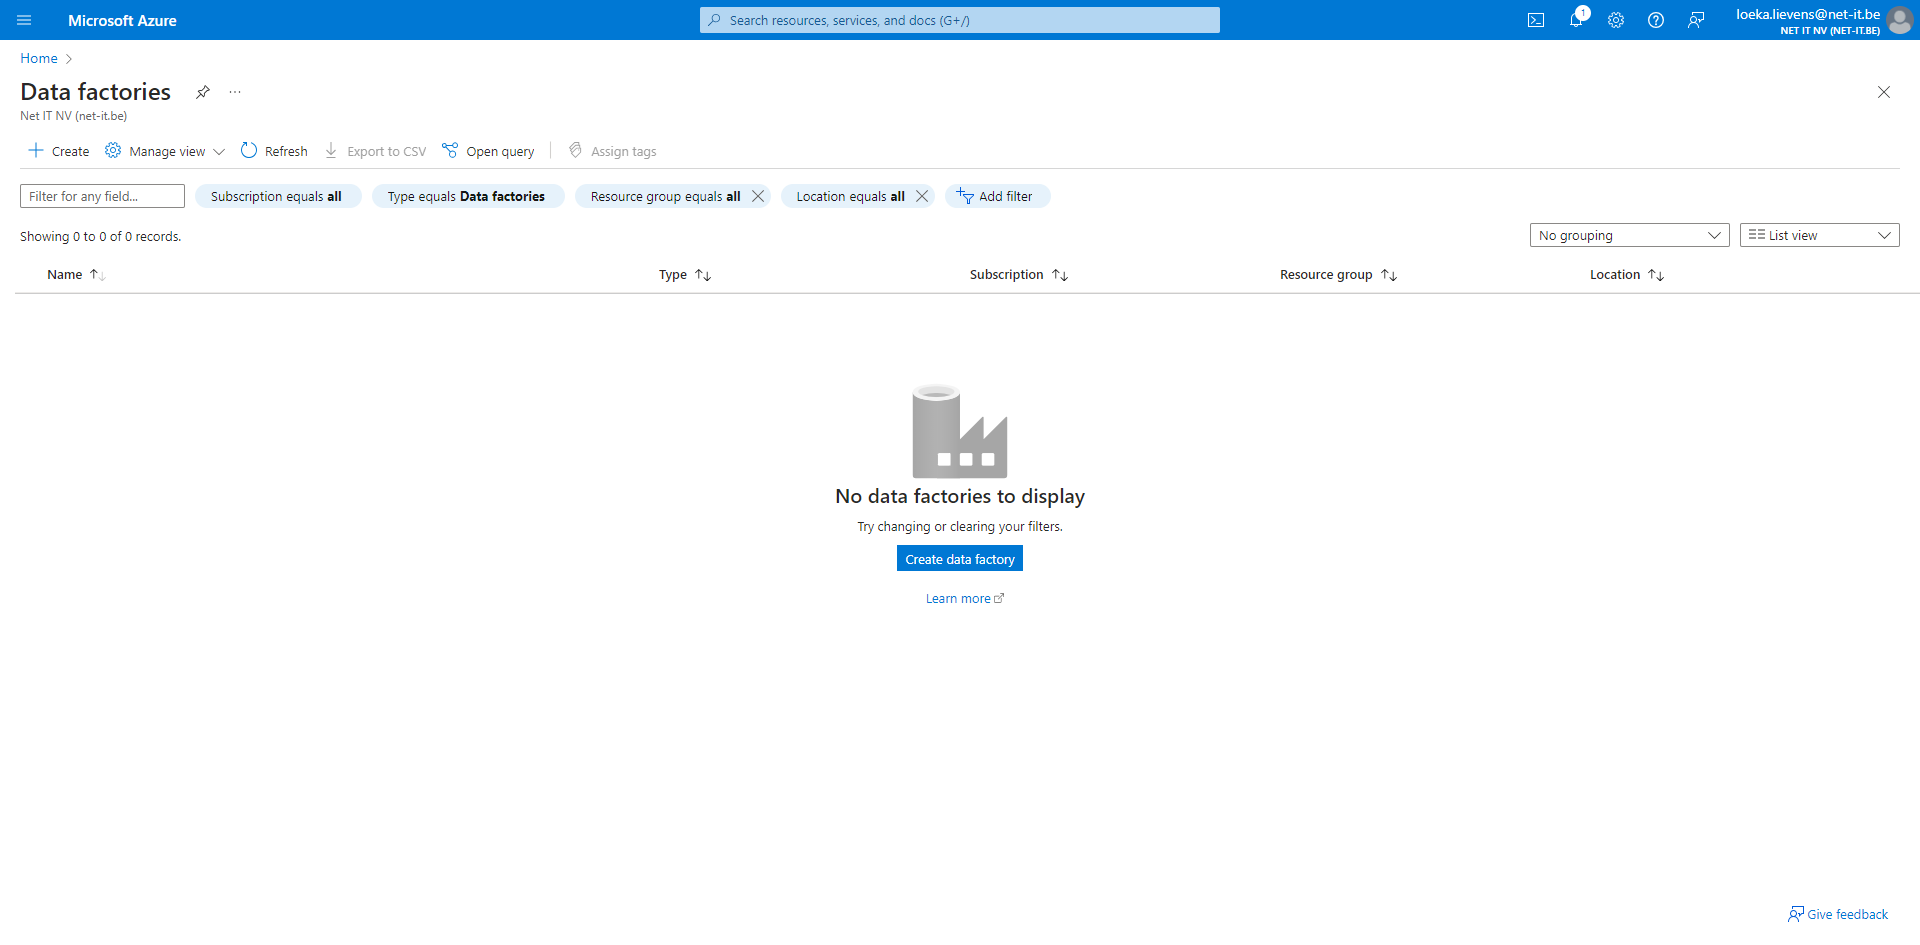
\includegraphics[width=0.6\textwidth]{./graphics/adf/initial.png}
    \footnote{Aanmaken van Azure Data Factory}
\end{center}

Door in Microsoft Azure naar Data Factories te navigeren kunnen we een nieuwe data factory gaan aanmaken.

\begin{center}
    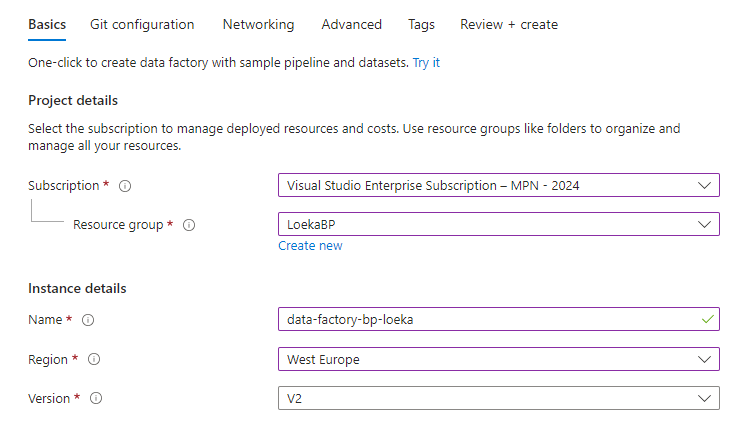
\includegraphics[width=0.6\textwidth]{./graphics/adf/initial_create.png}
    \footnote{Configuratie van Azure Data Factory}
\end{center}

% Resource group en subscription in literatuurstudie
Bij het aanmaken van een data factory moet er een subscription en resource group gekozen worden. Er kan een nieuwe resource group aangemaakt worden of een reeds bestaande gekozen worden. Daarnaast moet er een naam, gewenste regio en versie voor Data Factory gekozen worden. Git configuratie zal later aan bod komen. Data Factory kan nu aangemaakt worden.

\begin{center}
    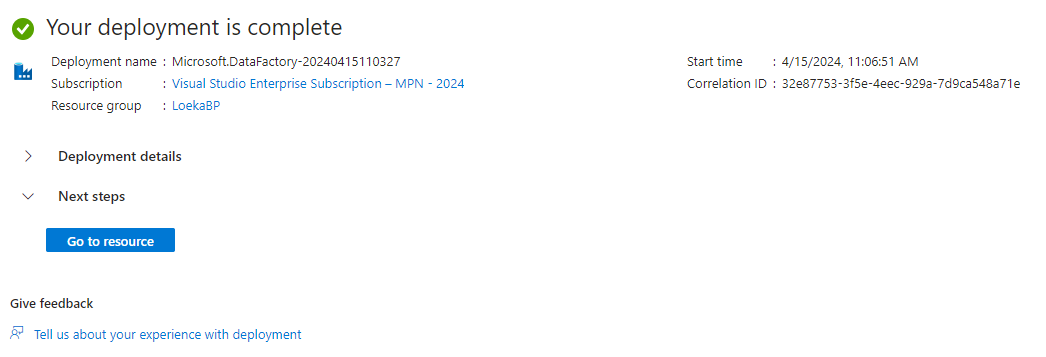
\includegraphics[width=0.6\textwidth]{./graphics/adf/deployment_complete_specific.png}
    \footnote{Deployment complete van Azure Data Factory}
\end{center}

Wanneer de resource is aangemaakt kan Azure Data Factory opgestart worden.

\subsubsection{Collaboration en source control}

Binnen Azure Data Factory kan er op 2 manieren samen gewerkt worden. 

\textbf{Roles en permissions}

\begin{center}
    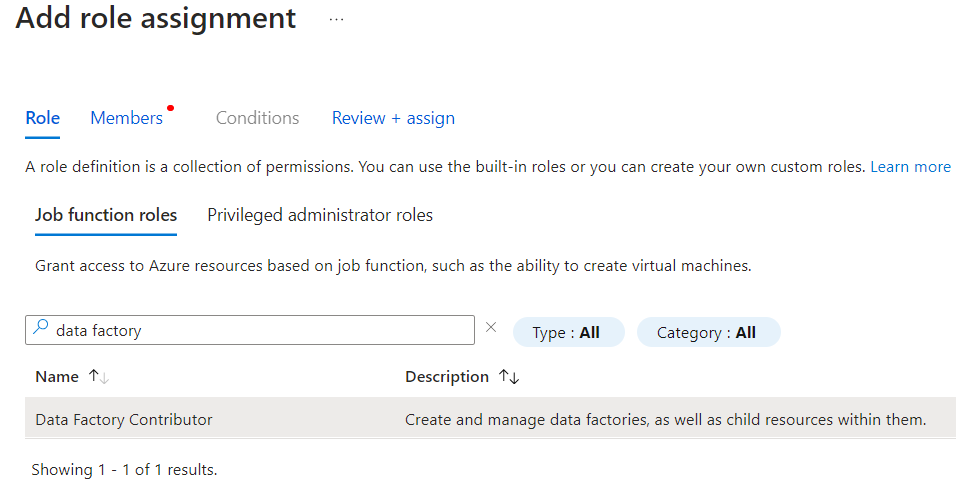
\includegraphics[width=0.6\textwidth]{./graphics/adf/adf_contributor.png}
    \footnote{Toewijzen van Data Factory Contributor Role}
\end{center}

Door de bij de resource group van de data factory de Data Factory Contributor role toe te wijzen kan men toegang geven tot volgende zaken:
\begin{itemize}
    \item Het aanmaken, wijzigen en verwijderen van data factories en child resources
    \item Deployment van Resource Manager templates
    \item Het managen van App Insight alerts voor Data Factory
    \item Het aanmaken van support tickets
\end{itemize}

\textbf{Source control}

Azure Data Factory laat het toe om een Git repository te configureren via Azure Repos of GitHub. 

\begin{center}
    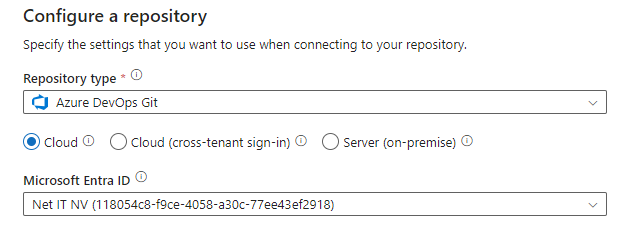
\includegraphics[width=0.6\textwidth]{./graphics/adf/setup_repository_2_specific.png}
    \footnote{Configuratie van Git in Azure Data Factory}
\end{center}

We kiezen voor Azure DevOps doordat er binnen Net IT hiermee gewerkt wordt.

\begin{center}
    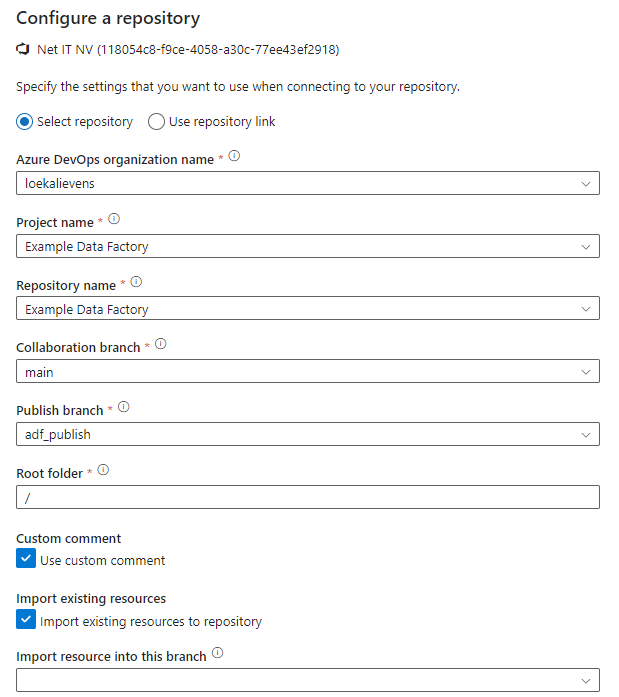
\includegraphics[width=0.6\textwidth]{./graphics/adf/setup_repository_3_specific.png}
    \footnote{Configuratie van Azure DevOps in Azure Data Factory}
\end{center}

De collaboration branch is de enigste branch waarbij de publish knop zichtbaar zal zijn. Door te werken met feature branches en hiermee pull requests te maken op de collaboration branch kan er dus samen gewerkt worden. De publish branch is de branch waar alle ARM templates van de gepubliceerde factory opgeslaan wordt.

\subsubsection{Ophalen van data uit Azure Data Lake}

Het ophalen van data uit Data Lake in Data Flow zal steeds op dezelfde manier gebeuren. 

\begin{center}
    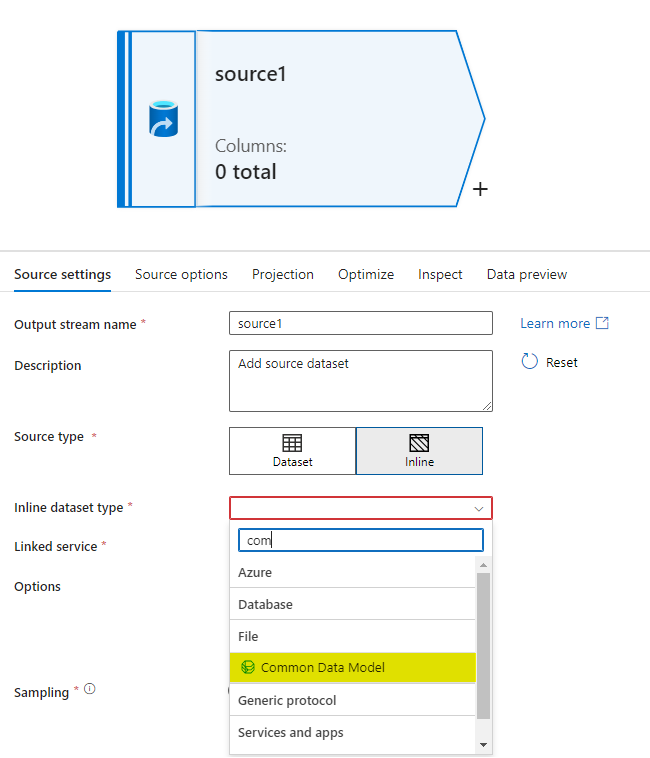
\includegraphics[width=0.6\textwidth]{./graphics/adf/source_table_1_specific.png}
    \footnote{Configuratie van source transformation}
\end{center}

Als source type zal er steeds gekozen worden voor inline. Dit doordat we slechts werken met één enkele dataflow en geen gedeelde datasets nodig hebben. Als inline data set type kiezen we voor Common Data Model.

\begin{center}%
    \centering
    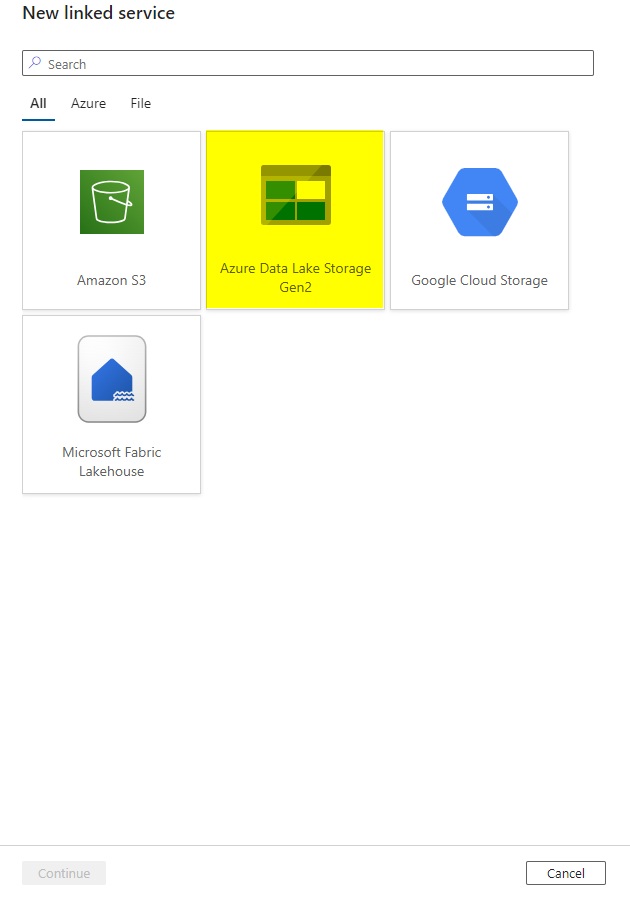
\includegraphics[width=0.4\textwidth]{./graphics/adf/source_table_2_specific}
    \hspace{0.1\textwidth}
    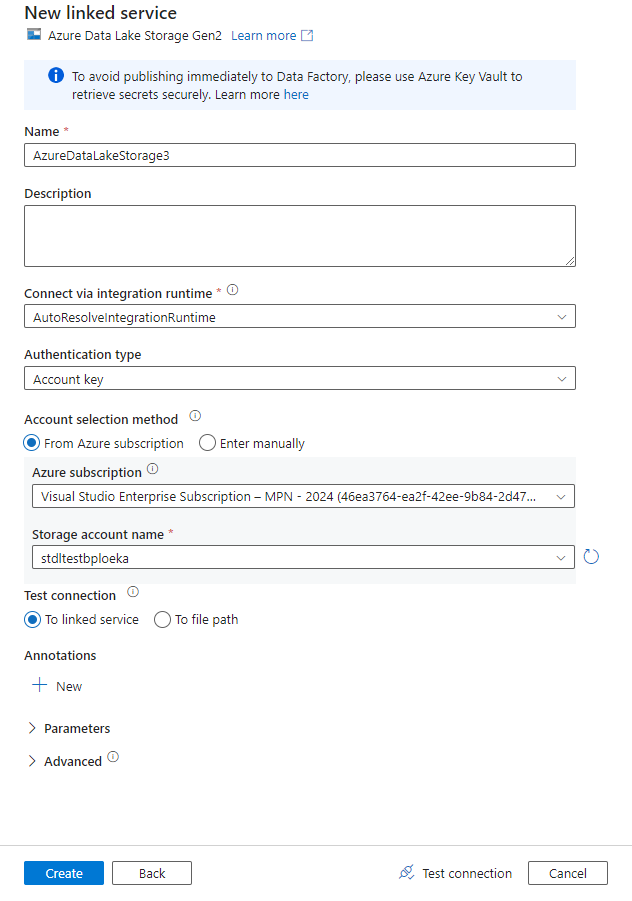
\includegraphics[width=0.4\textwidth]{./graphics/adf/source_table_3_specific}
    \footnote{Configuratie van linked service}
\end{center}

Er zal éénmalig een Linked Service aangemaakt moeten worden. Hierbij kiezen we voor Azure Data Lake Storage Gen2. We kunnen makkelijk gaan koppelen met de juiste data lake door een Azure Subscription en Storage account name aan te duiden. Door op `Test connection` te klikken kunnen we kijken of de connectie met data lake is gelukt. Door op `Create` te klikken hebben we nu een Linked Service die steeds bij elke Source gebruikt kan worden.

\textbf{Let op:} Doordat Git geen secrets opslaat is het aanbevolen om gebruik te maken van Azure Key Vault voor het opslaan van connection strings of passwords.

\begin{center}
    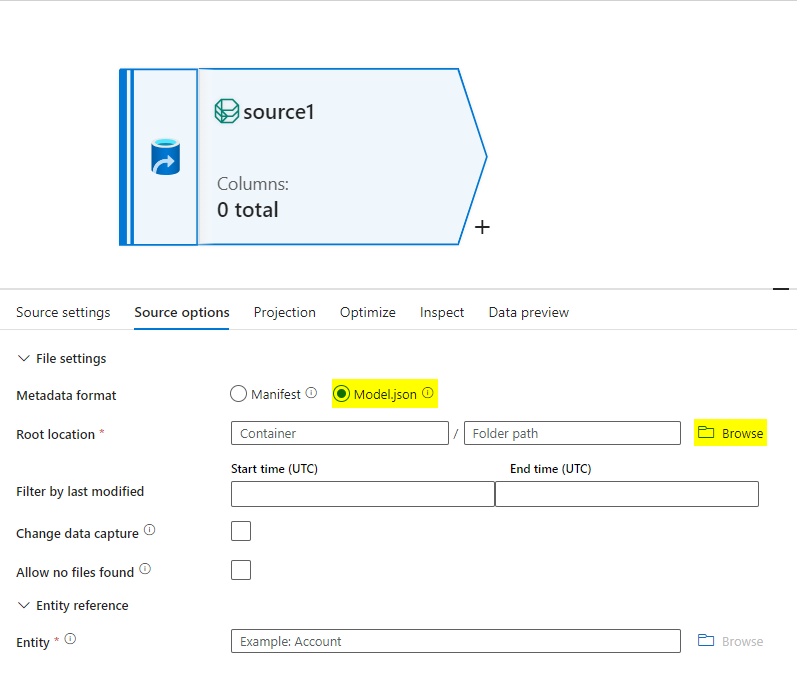
\includegraphics[width=0.6\textwidth]{./graphics/adf/source_table_4_specific.png}
    \footnote{Configuratie van source options}
\end{center}

Door naar `Source options` te gaan kunnen we `Model.json` gaan aanduiden. Door op `Browse` te klikken kunnen we aanduiden waar het Model.json bestand te vinden is in data lake.

\begin{center}
    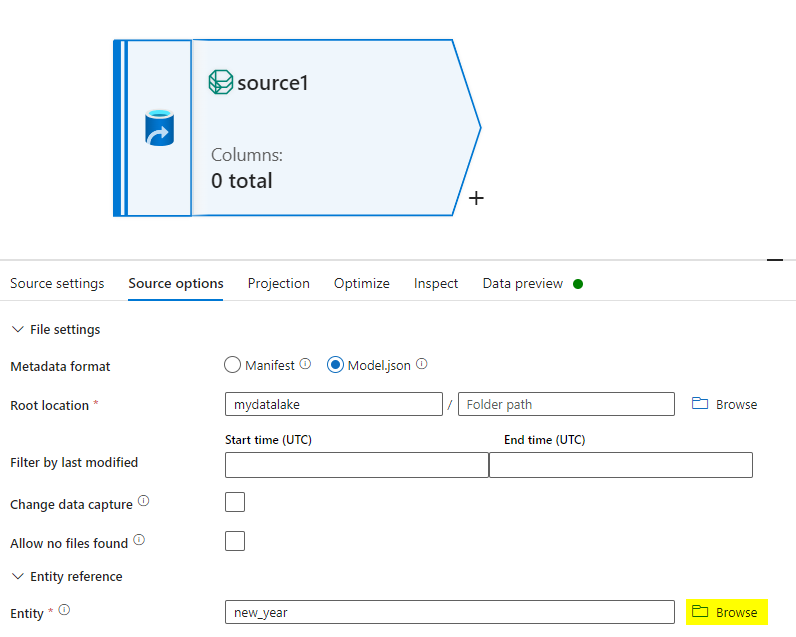
\includegraphics[width=0.6\textwidth]{./graphics/adf/source_table_5_specific.png}
    \footnote{Configuratie van source options}
\end{center}

Naast `Entity` kunnen we nu op `Browse` klikken om de gewenste entity te gaan importeren. Let op: hier voor zal Data flow debug aan moeten staan.

\begin{center}
    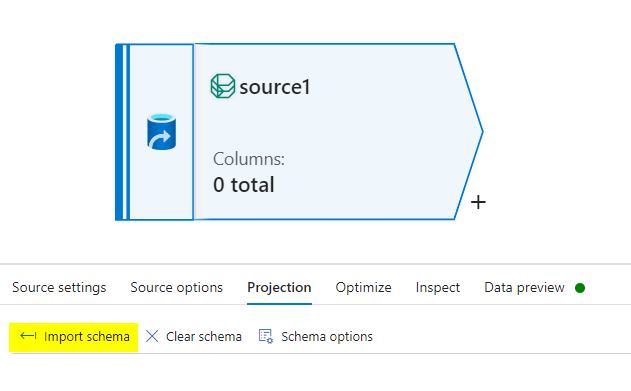
\includegraphics[width=0.6\textwidth]{./graphics/adf/source_table_6_specific.png}
    \footnote{Configuratie van projection}
\end{center}

Door naar `Projection` te gaan kunnen we nu op `Import schema` klikken.

\begin{center}
    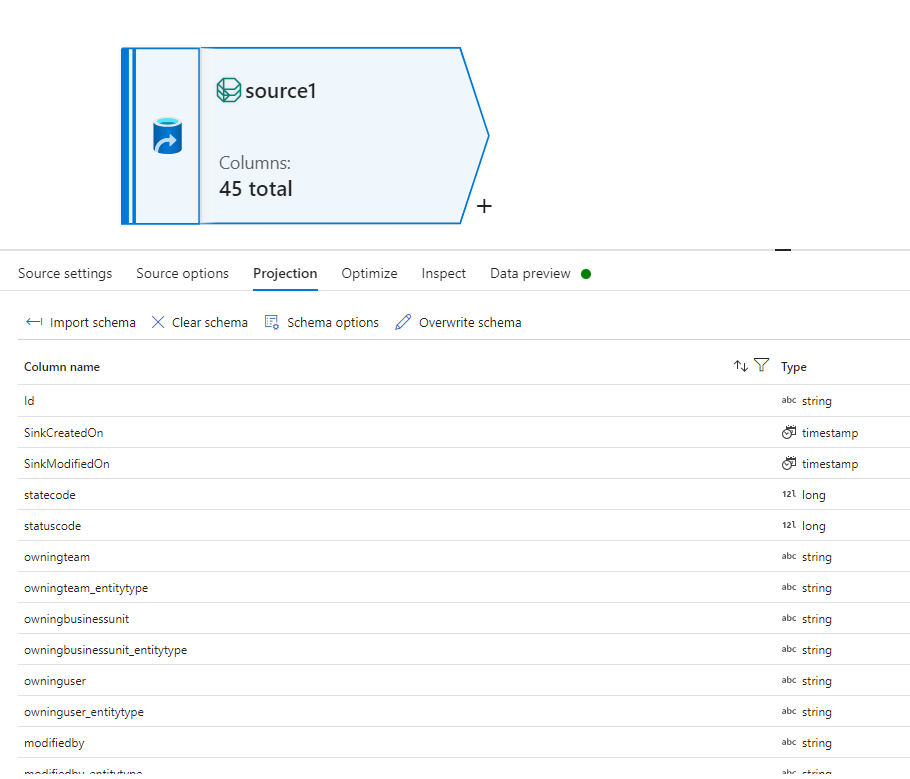
\includegraphics[width=0.6\textwidth]{./graphics/adf/source_table_7_specific.png}
    \footnote{Configuratie van projection}
\end{center}

De foto hierboven toont een voorbeeld van een geïmporteerd schema.

\begin{center}
    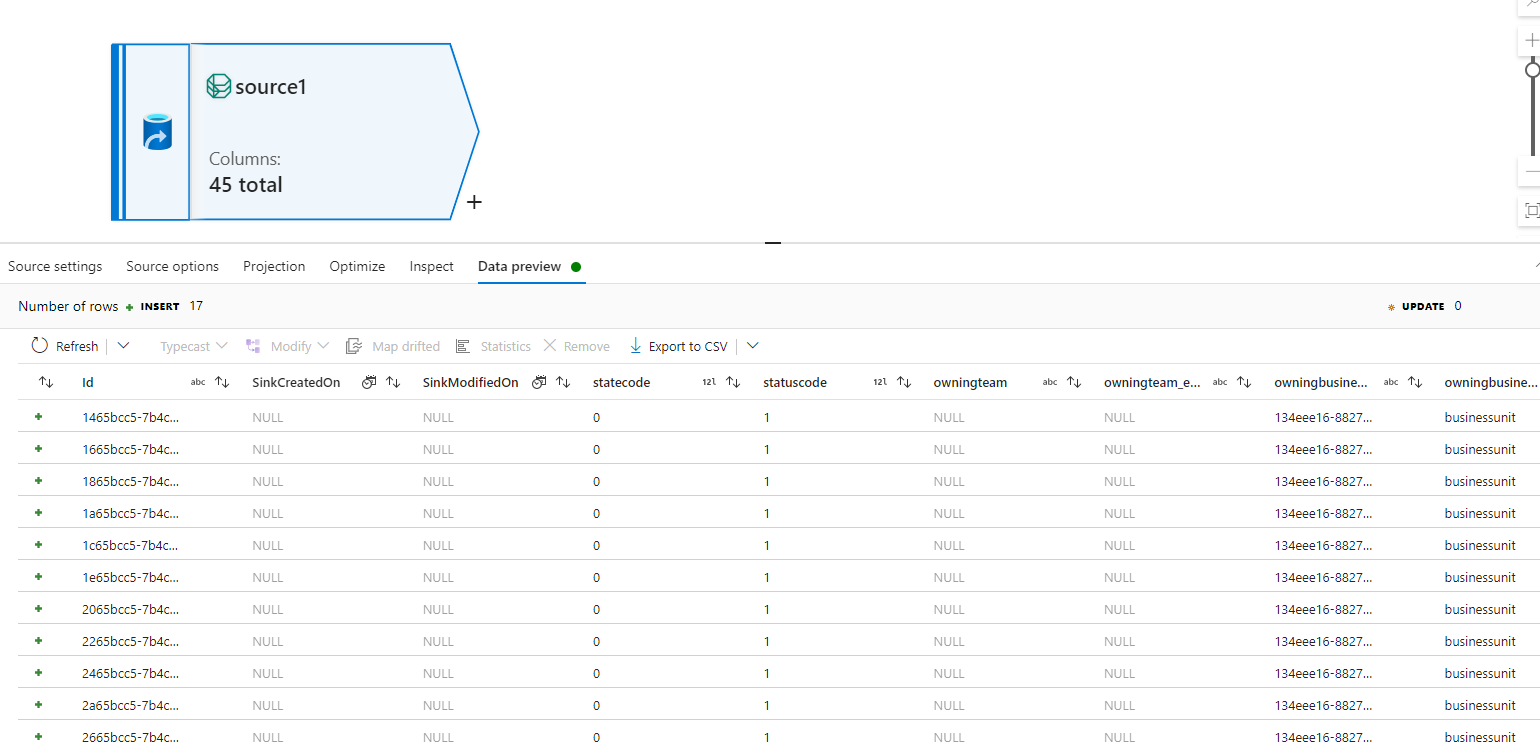
\includegraphics[width=0.6\textwidth]{./graphics/adf/source_table_8_specific.png}
    \footnote{Data preview}
\end{center}

Wanneer we naar `Data preview` gaan kunnen we een preview zien van de data uit de gekozen tabel.

\subsubsection{Belangrijkste transformaties}

\textbf{Determinatie van welke groepen de premie in hun bestand krijgen}

\begin{center}
    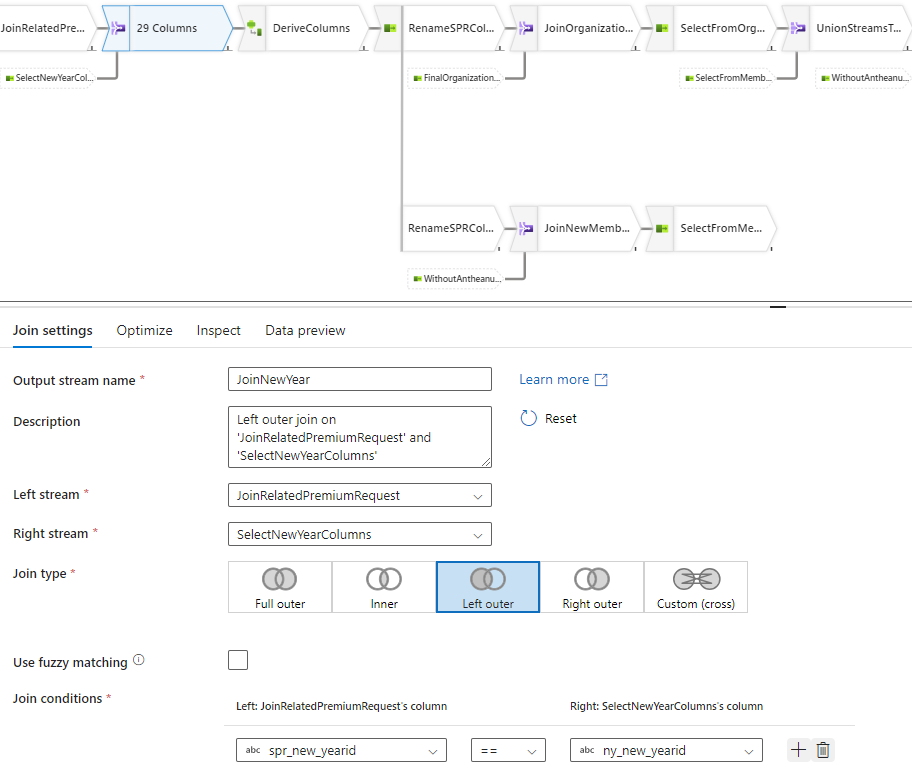
\includegraphics[width=0.6\textwidth]{./graphics/adf/bepalen_groep_1.png}
    \footnote{Join van de tabel `new\_year` op de tabel `new\_syndicalpremiumrequest`}
\end{center}

De tabel `new\_syndicalpremiumrequest` heeft een kolom `spr\_new\_yearid`. Om te gaan bepalen wat het referentiejaar van deze premie is zal dus de tabel `new\_year` op de tabel `new\_syndicalpremiumrequest` gejoind moeten worden aan de hand van dit id.


\begin{center}
    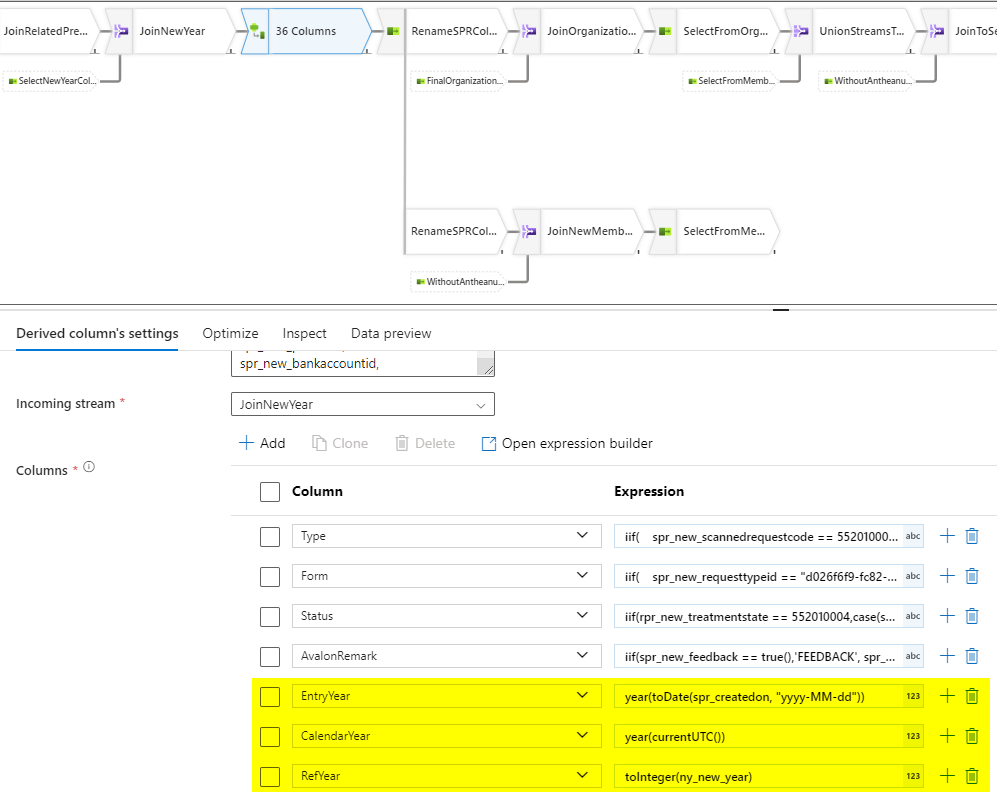
\includegraphics[width=0.6\textwidth]{./graphics/adf/bepalen_groep_2.png}
    \footnote{Derive EntryYear, CalendarYear en RefYear op de tabel `new\_syndicalpremiumrequest`}
\end{center}

Voor het groepen moeten hebben we 3 nieuwe kolommen nodig. Als eerste hebben we het EntryYear nodig, dit is het jaartal van `spr\_createdon`, de datum wanneer de record is aangemaakt. Daarnaast hebben we CalendarYear nodig, dit is het jaartal van de huidige datum. En ten slotte hebben we RefYear nodig, dit is het jaartal van de tabel `new\_year` die net gejoind is geweest.

\begin{center}
    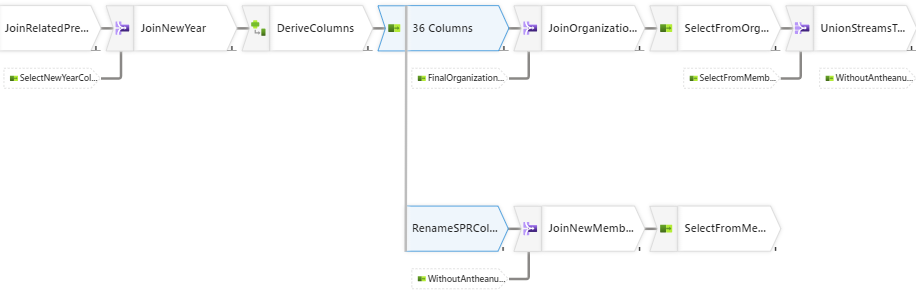
\includegraphics[width=0.6\textwidth]{./graphics/adf/bepalen_groep_3.png}
    \footnote{Hernoemen van `new\_syndicalpremiumrequest` kolommen en splitsing in twee apparte branches}
\end{center}

Vervolgens worden bepaalde kolommen van naam hernoemt. Welke kolommen dit zijn is onbelangrijk voor deze transformatie. Wat wel belangrijk is dat de pipeline zich nu opsplitst in twee apparte branches. Dit doordat er 2 inner joins zullen gebeuren.

\begin{center}
    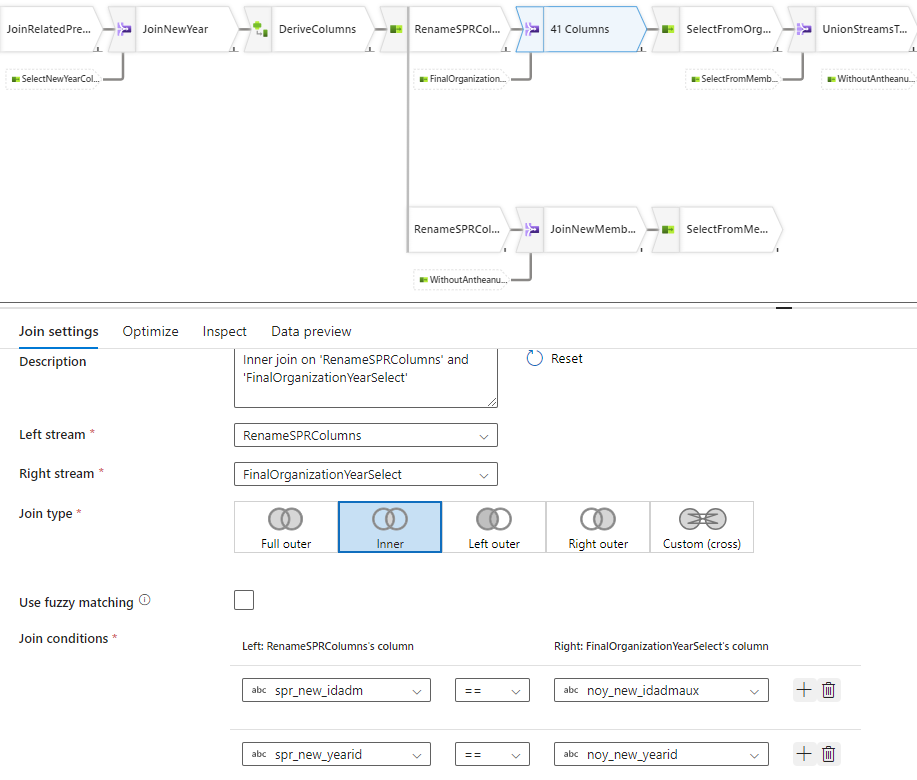
\includegraphics[width=0.6\textwidth]{./graphics/adf/bepalen_groep_4.png}
    \footnote{Inner join van `new\_organizationyear` op de tabel `new\_syndicalpremiumrequest`}
\end{center}

Er gebeurt nu een inner join van de tabel `new\_organizationyear` op de tabel `new\_syndicalpremiumrequest`. Hierbij wordt er aan de hand van IDADM en het id van het referentiejaar gejoind.

\begin{center}
    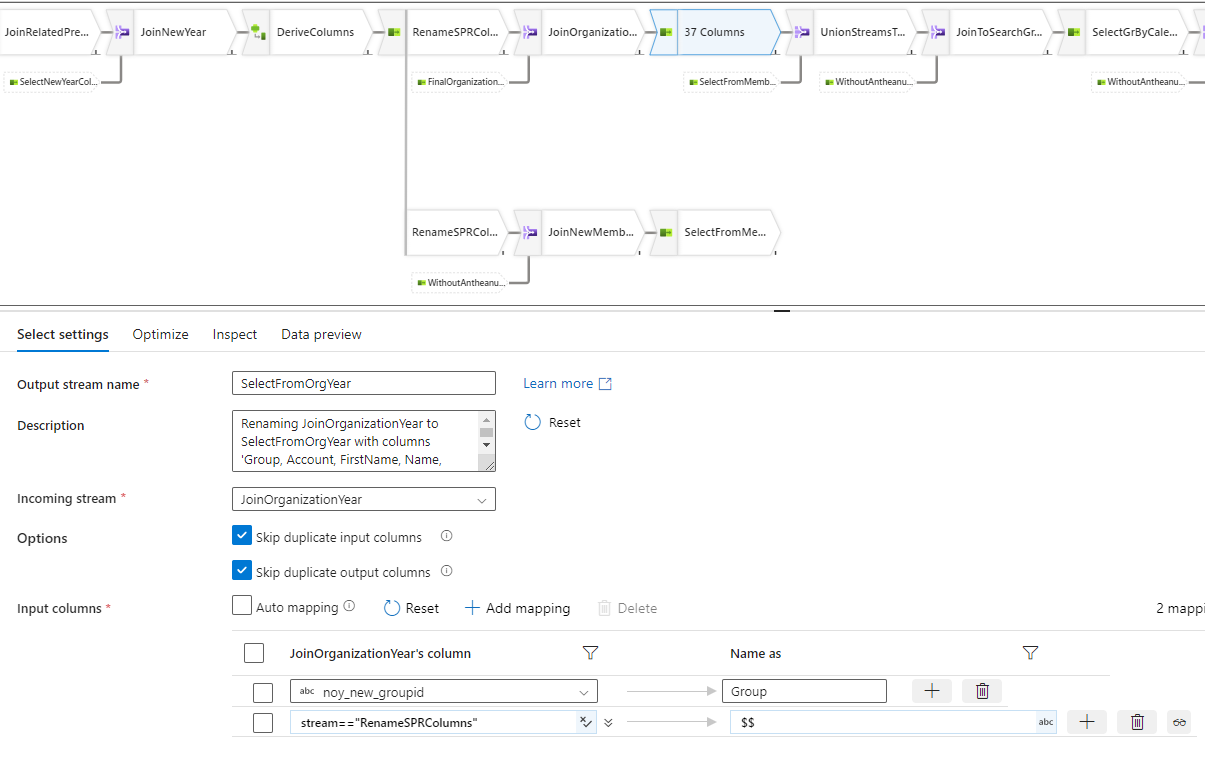
\includegraphics[width=0.6\textwidth]{./graphics/adf/bepalen_groep_5.png}
    \footnote{Selecteren en hernoemen van kolommen op de tabel `new\_syndicalpremiumrequest`}
\end{center}

Vervolgens worden alle kolommen die er voor de join waren geselecteerd. Daarnaast wordt er één kolom `noy\_new\_groupid` geselecteerd en hernoemd naar `Group`.

\begin{center}
    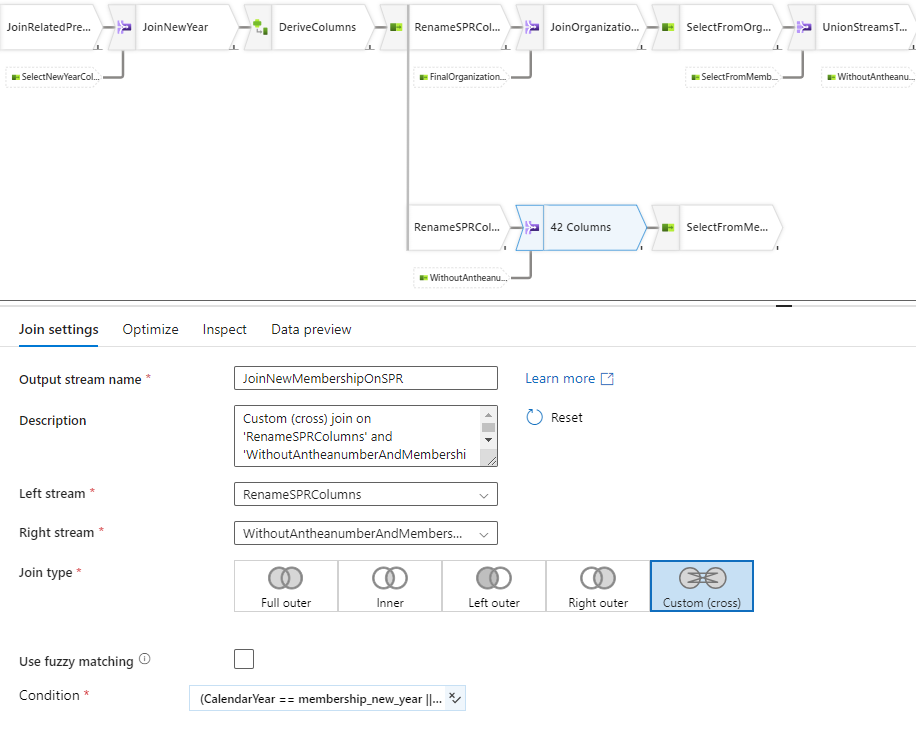
\includegraphics[width=0.6\textwidth]{./graphics/adf/bepalen_groep_6.png}
    \footnote{Custom (cross) join van `new\_membership` op de tabel `new\_syndicalpremiumrequest`}
\end{center}

Bij de tweede branch wordt de tabel `new\_membership` gejoind op de tabel `new\_syndicalpremiumrequest`. Er wordt gebruik gemaakt van een custom (cross) join doordat er OR condities worden gebruikt. 

\begin{center}
    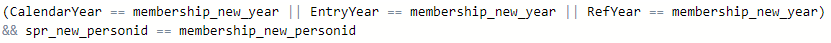
\includegraphics[width=0.6\textwidth]{./graphics/adf/bepalen_groep_7.png}
    \footnote{Conditie van de custom (cross) join van `new\_membership` op de tabel `new\_syndicalpremiumrequest`}
\end{center}

In de conditie van de custom (cross) join wordt er vergeleken of CalendarYear, EntryYear of RefYear overeenkomt met het jaartal van de membership. Daarnaast wordt er ook gekeken of personid overeen komt.

\begin{figure}[H]
    \centering
    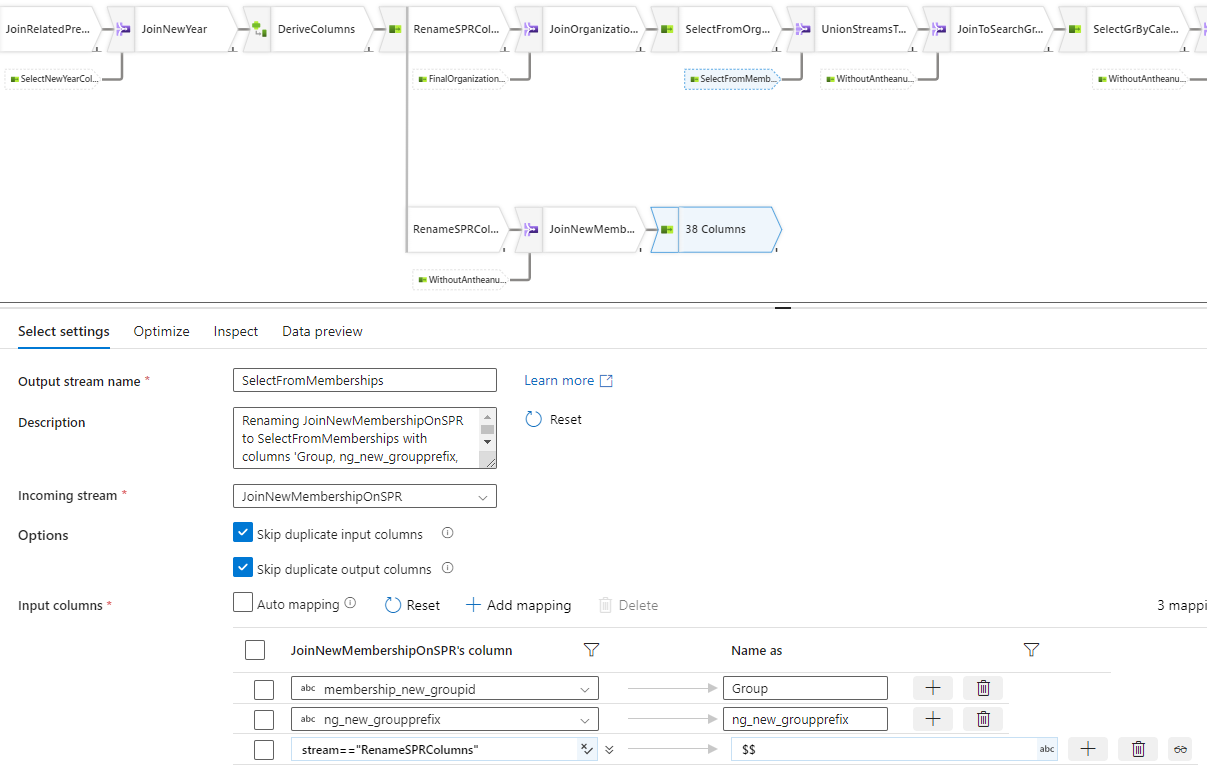
\includegraphics[width=0.6\textwidth]{./graphics/adf/bepalen_groep_8.png}
    \caption{Selecteren en hernoemen van kolommen op de tabel `new\_syndicalpremiumrequest`}
    \label{fig:bepalengroep}
\end{figure}

Ook na deze join worden alle kolommen die er voor de join waren geselecteerd. Daarnaast wordt er 1 kolom `membership\_new\_groupid` geselecteerd en hernoemd naar `Group`. Ten slotte wordt de kolom `ng\_new\_groupprefix` geselecteerd maar dit heeft te maken met een andere transformatie.

\begin{center}
    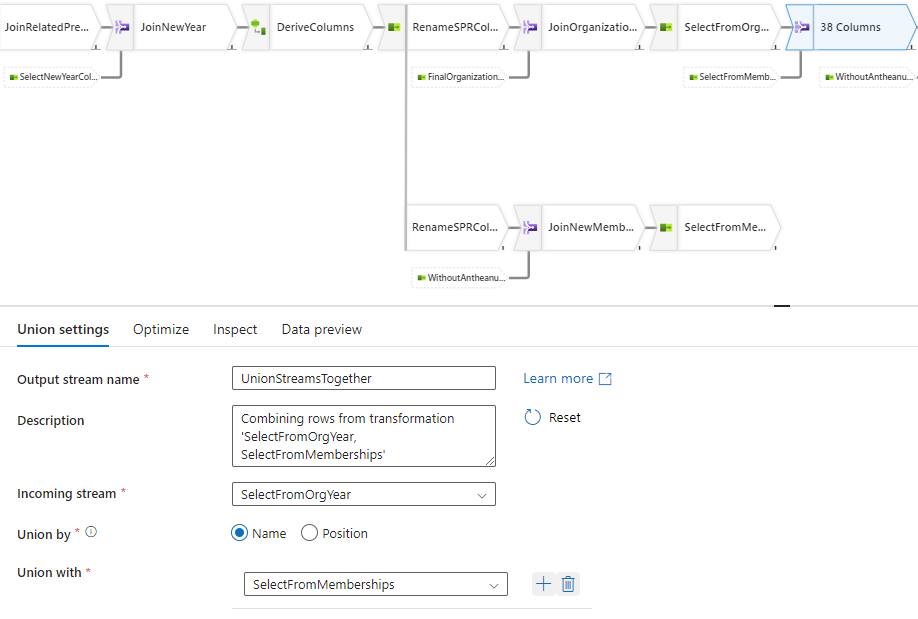
\includegraphics[width=0.6\textwidth]{./graphics/adf/bepalen_groep_9.png}
    \footnote{Union van twee branches}
\end{center}

Beide branches hebben nu dezelfde kolommen met een extra kolom `Group`. Daarnaast heeft de onderste branch nog één extra kolom `ng\_new\_groupprefix`. De beide branches worden nu samen gevoegd met behulp van een union. De bovenste branch die de kolom `ng\_new\_groupprefix` niet heeft zal voor deze kolom de waarde `NULL` krijgen in de records komende van deze branch. 

\begin{figure}[H]
    \centering
    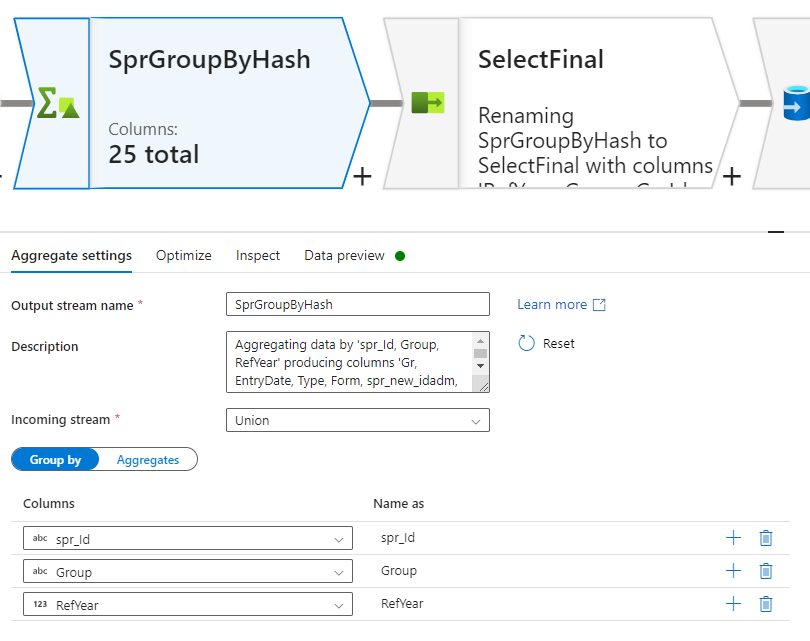
\includegraphics[width=0.6\textwidth]{./graphics/adf/group_by_1.png}
    \caption{Group by `spr\_Id`, `Group` en `RefYear` in `new\_syndicalpremiumrequest`}
    \label{fig:groupby}
\end{figure}

Om te voorkomen dat een premie twee keer in het zelfde bestand terecht komt voor een bepaalde groep en referentiejaar zal er op het einde van de pipeline geaggregeerd worden op basis van id van de premie, groep en referentiejaar.

\begin{center}
    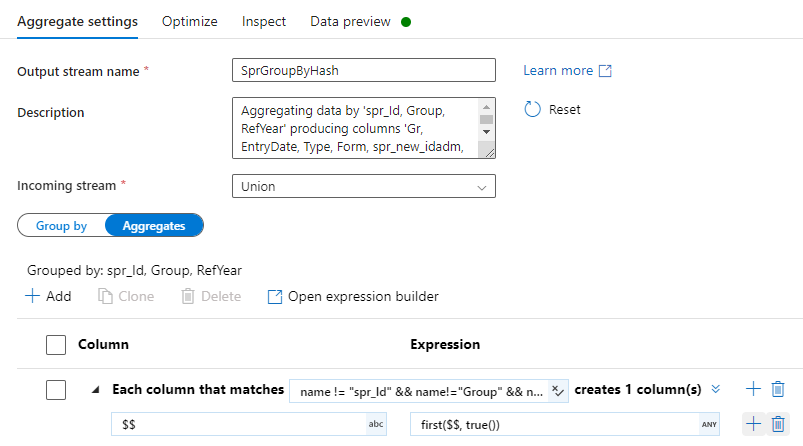
\includegraphics[width=0.6\textwidth]{./graphics/adf/group_by_2.png}
    \footnote{Group by `spr\_Id`, `Group` en `RefYear` in `new\_syndicalpremiumrequest`}
\end{center}

\begin{center}
    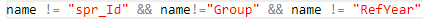
\includegraphics[width=0.6\textwidth]{./graphics/adf/group_by_3.png}
    \footnote{Group by `spr\_Id`, `Group` en `RefYear` in `new\_syndicalpremiumrequest`}
\end{center}

Voor alle kolommen behalve de kolommen die in de `Group by` gebruikt worden zal de aggregatiefunctie `first` gebruikt worden. De tweede parameter `true()` wordt gebruikt om aan te geven dat NULL waardes genegeerd moeten worden. Dit zal dus resulteren in de eerste waarde die niet NULL is van de kolom groep. Indien alle waardes NULL zijn zal dit wel in NULL resulteren.


% TODO group by uitleggen

\textbf{Bepalen van de kolom `Gr` voor een premie}

\begin{center}
    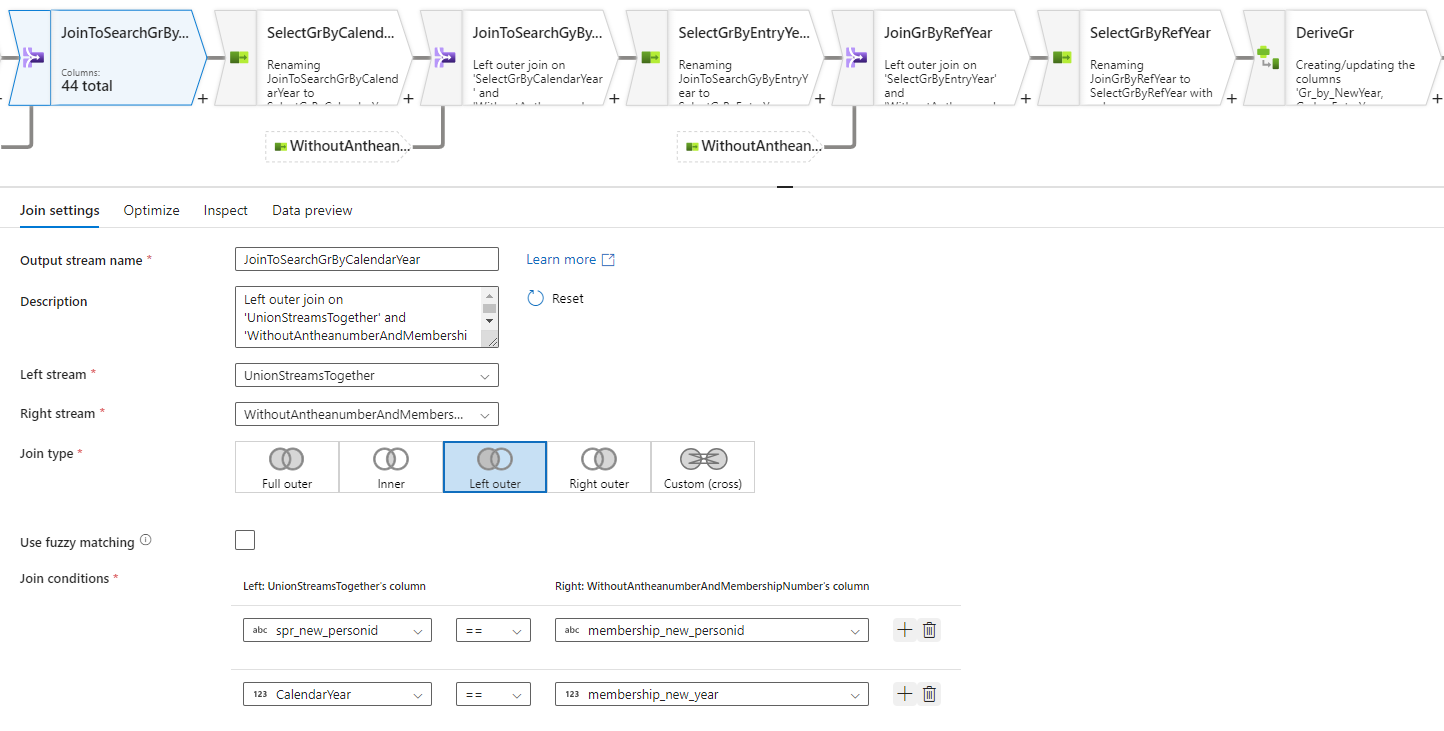
\includegraphics[width=0.9\textwidth]{./graphics/adf/gr_1.png}
    \footnote{Joinen van de tabel `new\_membership` op de tabel `new\_syndicalpremiumrequest`}
\end{center}

De tabel `new\_membership` wordt gejoind op de tabel `new\_syndicalpremiumrequest`. Dit gebeurd aan de hand van `new\_personid` en het kalenderjaar van de premie.

\begin{center}
    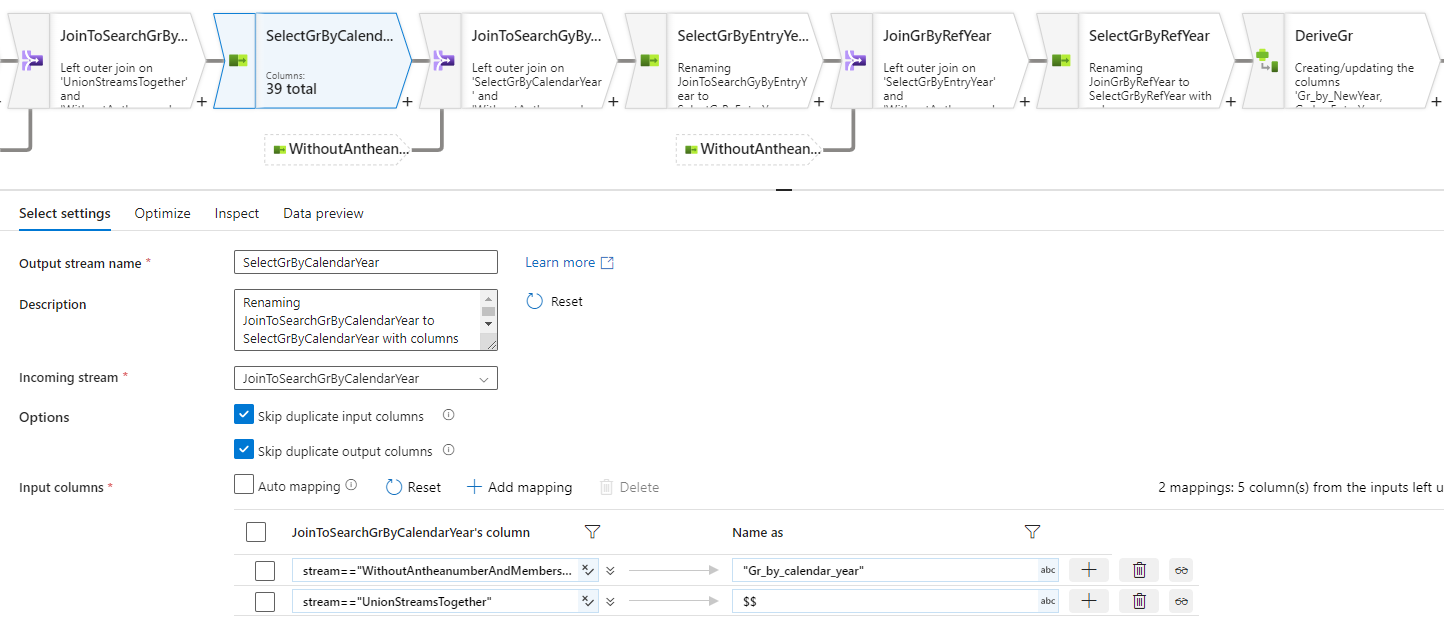
\includegraphics[width=0.9\textwidth]{./graphics/adf/gr_2.png}
    \footnote{Selecteren van de juiste kolommen in `new\_syndicalpremiumrequest`}
\end{center}

De kolommen die reeds bestonden voor de join worden geselecteerd. Daarnaast wordt de kolom `ng\_new\_groupprefix` geselecteerd en hernoemd naar `Gr\_by\_calendar\_year`.

\begin{center}
    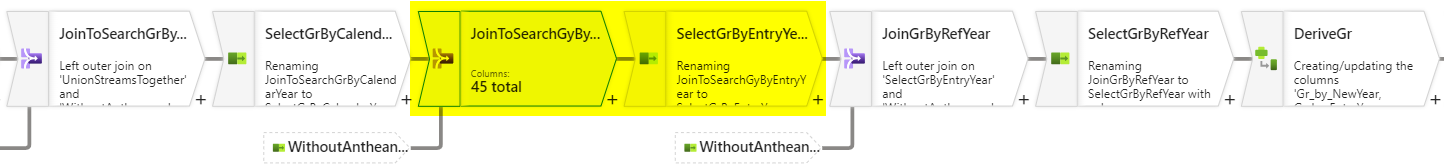
\includegraphics[width=0.9\textwidth]{./graphics/adf/gr_3.png}
    \footnote{Herhalen van transformaties}
\end{center}

Dezelfde transformaties gebeuren maar deze keer aan de hand van `EntryYear`. Ook hier worden de reeds bestaande kolommen geselecteerd en wordt de nieuwe kolom `ng\_new\_groupprefix` hernoemd naar `Gr\_by\_EntryYear`.

\begin{center}
    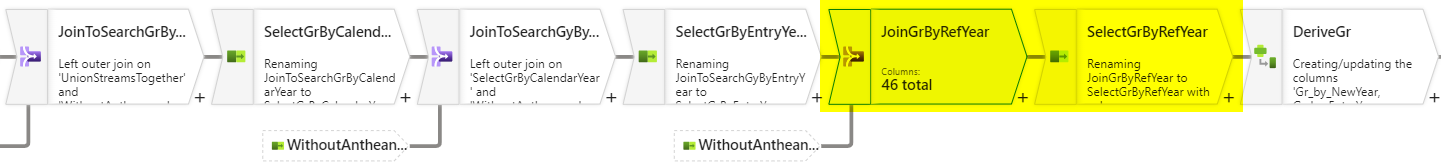
\includegraphics[width=0.9\textwidth]{./graphics/adf/gr_4.png}
    \footnote{Herhalen van transformaties}
\end{center}

Ook voor `RefYear` zullen deze transformaties gebeuren, resulterend in een nieuwe kolom `Gr\_by\_NewYear`.

\begin{center}
    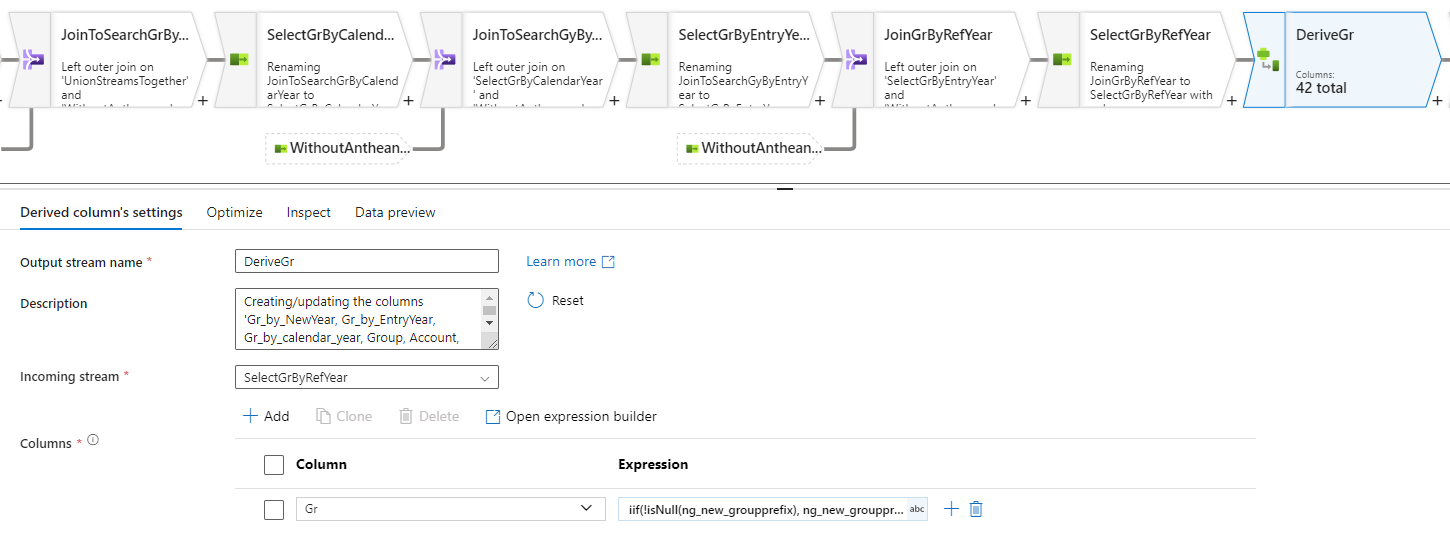
\includegraphics[width=0.9\textwidth]{./graphics/adf/gr_5.png}
    \footnote{Bepalen van `Gr` in `new\_syndicalpremiumrequest`}
\end{center}

We hebben nu een group prefix reeds komende uit een andere transformatie \ref{fig:bepalengroep} en group prefixes komende uit de joins die we hebben uitgevoerd.

\begin{minted}{text}
iif(!isNull(ng_new_groupprefix), ng_new_groupprefix, 
    iif(!isNull(Gr_by_calendar_year), Gr_by_calendar_year,
        iif(!isNull(Gr_by_EntryYear), Gr_by_EntryYear,
            iif(!isNull(Gr_by_NewYear), Gr_by_NewYear, toString(null())))))
\end{minted}

Om de kolom `Gr` te bepalen zal er gezocht worden naar de eerste kolom die niet NULL is startende van uit `ng\_new\_groupprefix` waarbij er vervolgens gekeken wordt naar `Gr\_by\_calendaryear`, `Gr\_by\_EntryYear` en `Gr\_by\_NewYear`.

Ook voor deze transformatie is het belangrijk dat er geaggregeerd wordt zoals bij Figuur \ref{fig:groupby} om te voorkomen dat dezelfde premie twee keer in een groep voor een bepaald jaartal terecht komt.

\textbf{Bepalen van de kolommen `AntheaNumber` en `MembershipNumber` voor een premie}

\begin{center}
    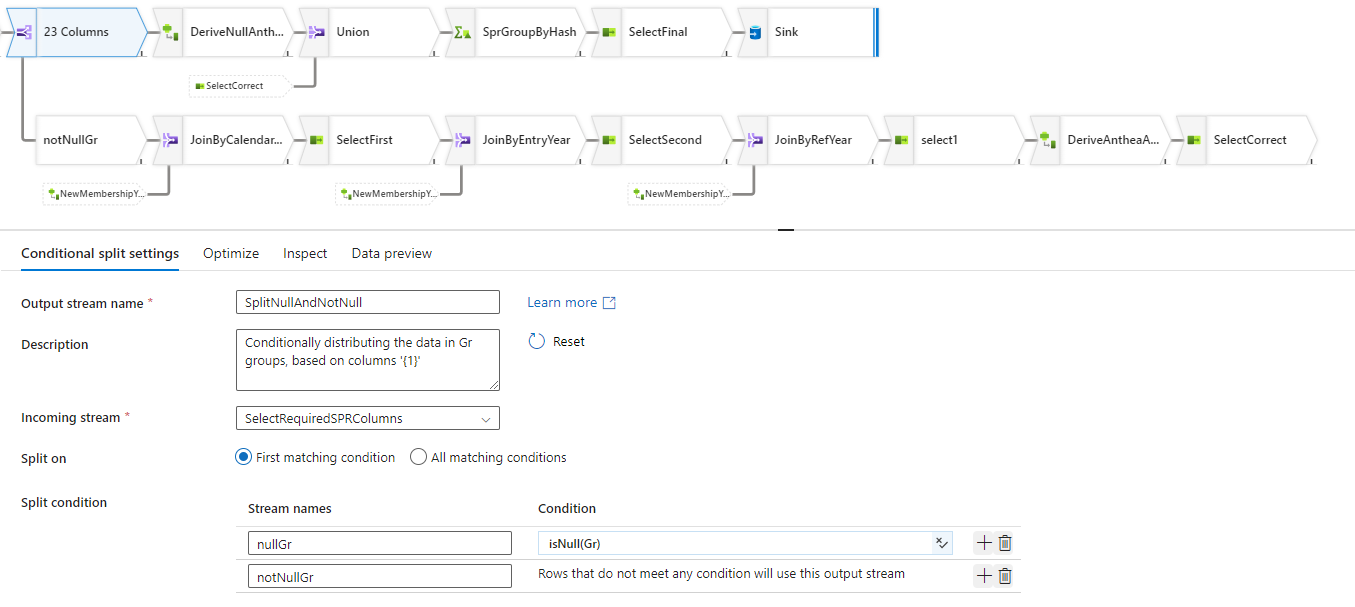
\includegraphics[width=0.9\textwidth]{./graphics/adf/member_1.png}
    \footnote{Conditional split op `new\_syndicalpremiumrequest`}
\end{center}

De pipeline zal splitten in twee branches met behulp van een conditional split. Alle rijen waarbij de kolom `Gr` NULL is zullen boven verder gaan. Alle rijen waarbij de kolom `Gr` niet NULL is zullen onderaan verder gaan.

\begin{center}
    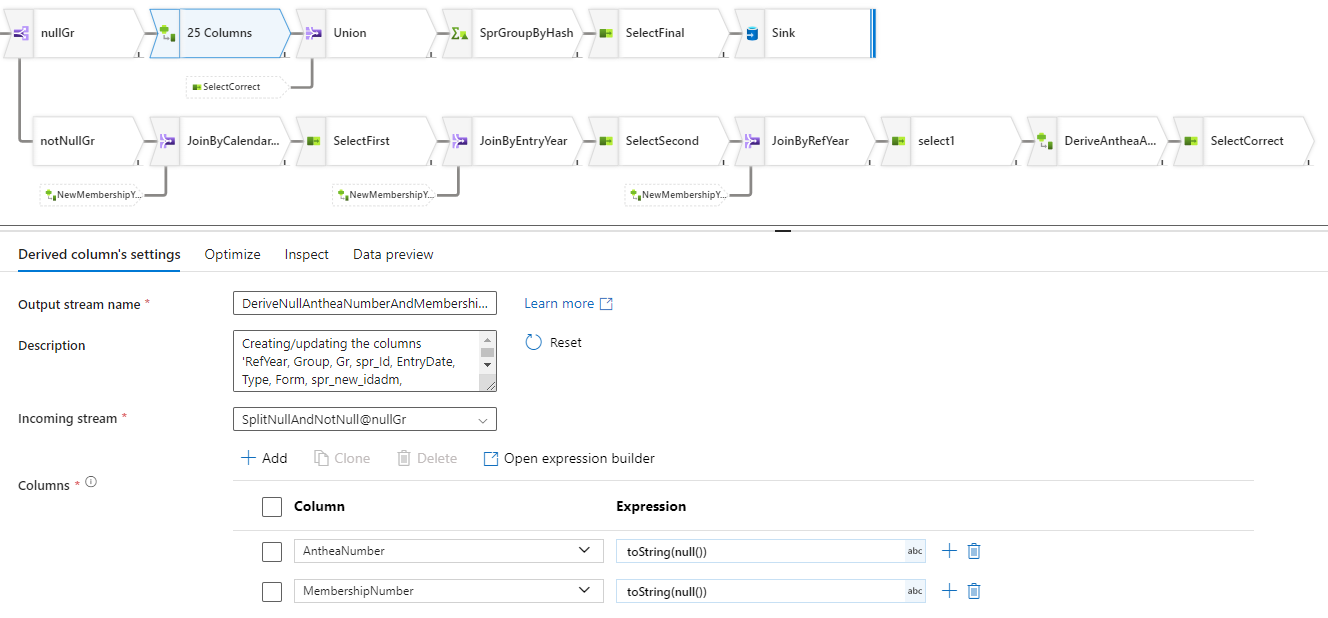
\includegraphics[width=0.9\textwidth]{./graphics/adf/member_2.png}
    \footnote{Derive `AntheaNumber` en `MembershipNumber` op de tabel `new\_syndicalpremiumrequest`}
\end{center}

Voor de rijen waarbij de kolom `Gr` NULL was zullen de kolommen `AntheaNumber` en `MembershipNumber` ook NULL zijn.

\begin{center}
    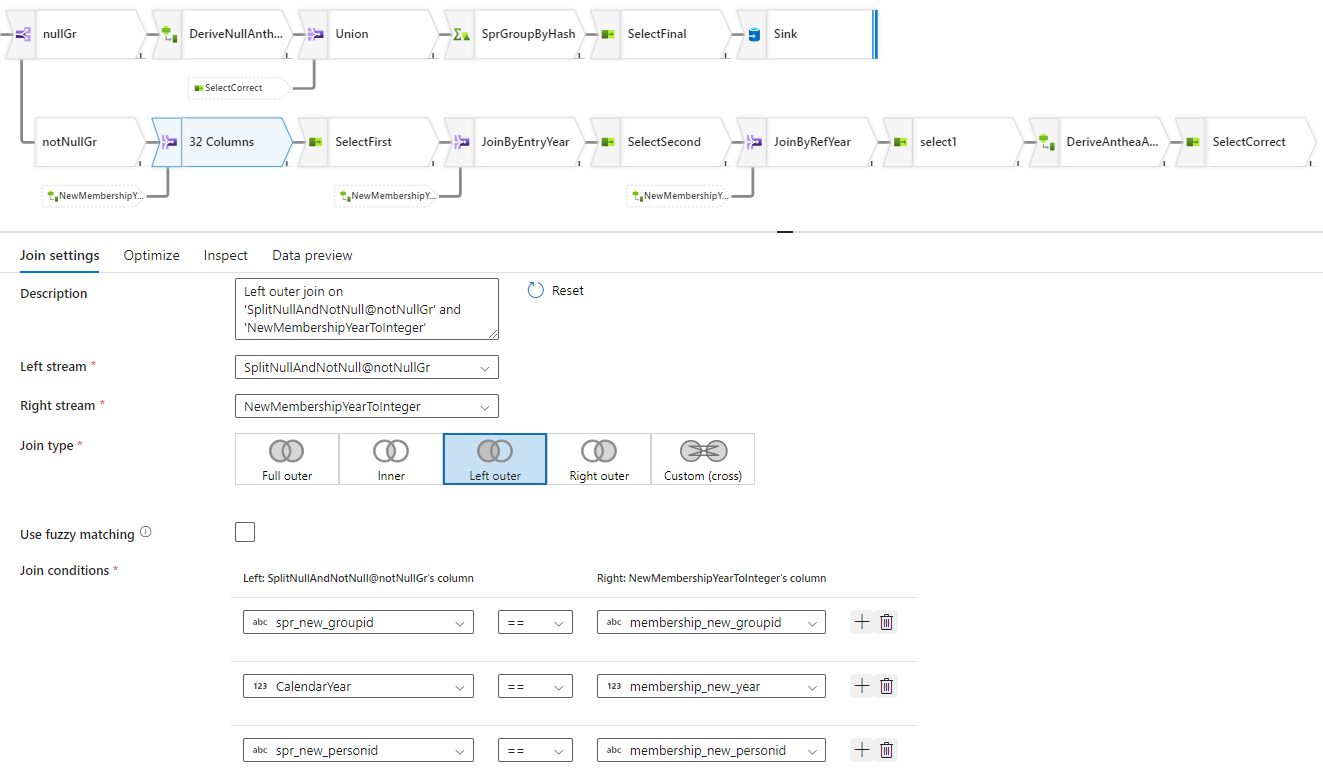
\includegraphics[width=0.9\textwidth]{./graphics/adf/member_3.png}
    \footnote{Join van de tabel `new\_membership` op de tabel `new\_syndicalpremiumrequest` aan de hand van `new\_groupid`, `new\_personid` en `CalendarYear`}
\end{center}

Voor de rijen waarbij de kolom `Gr` niet NULL was zal de tabel `new\_membership` gejoind worden. Hierbij wordt er gebruik gemaakt van `group\_id`, `new\_personid` en `CalendarYear`.

\begin{center}
    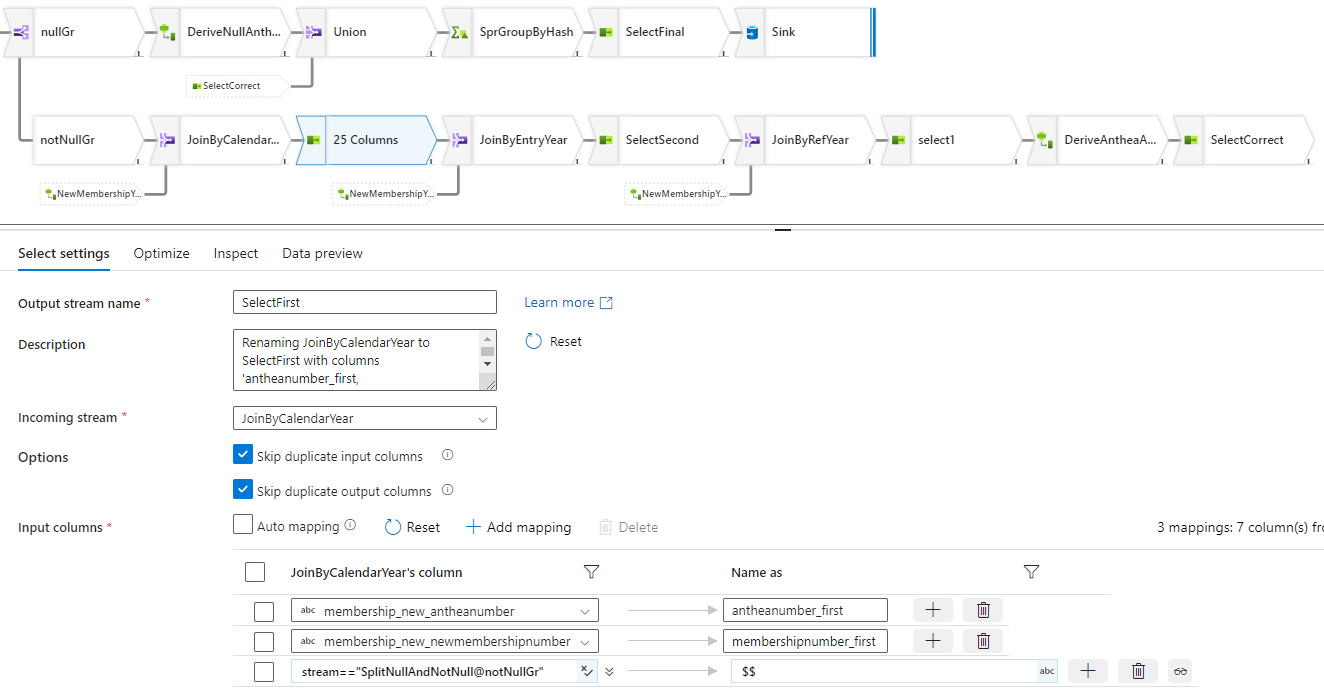
\includegraphics[width=0.9\textwidth]{./graphics/adf/member_4.png}
    \footnote{Select op de tabel `new\_syndicalpremiumrequest`}
\end{center}

Alle kolommen die er voor de join waren zullen opnieuw geselecteerd worden. Daarnaast worden `membership\_new\_antheanumber` en `membership\_new\_newmembershipnumber` geselecteerd en hernoemd naar `antheanumber\_first` en `membershipnumber\_first`.

\begin{center}
    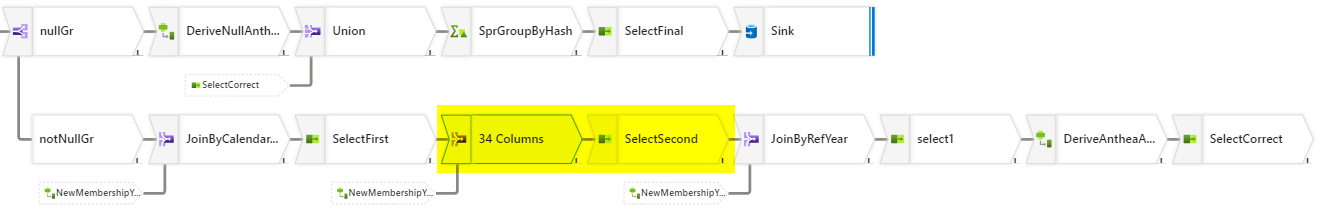
\includegraphics[width=0.9\textwidth]{./graphics/adf/member_5.png}
    \footnote{Join van de tabel `new\_membership` op de tabel `new\_syndicalpremiumrequest` aan de hand van `new\_groupid`, `new\_personid` en `EntryYear`}
\end{center}

De vorige twee transformatie gebeuren opnieuw maar deze keer wordt er gebruik gemaakt van `EntryYear` in plaats van `CalendarYear`.

\begin{center}
    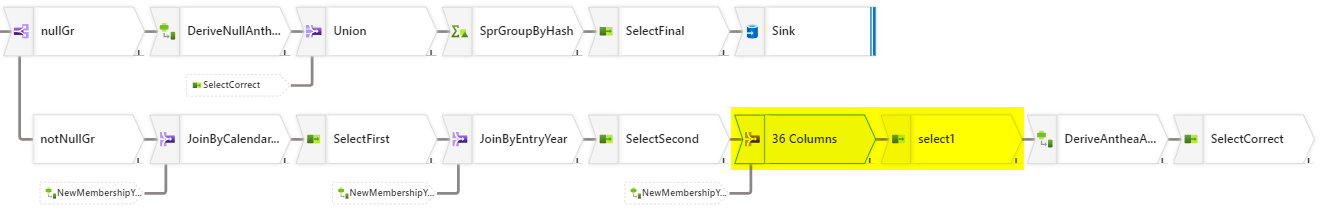
\includegraphics[width=0.9\textwidth]{./graphics/adf/member_6.png}
    \footnote{Join van de tabel `new\_membership` op de tabel `new\_syndicalpremiumrequest` aan de hand van `new\_groupid`, `new\_personid` en `RefYear`}
\end{center}

Ook zal voor `RefYear` in plaats van `CalendarYear` deze transformaties opnieuw gebeuren.

\begin{center}
    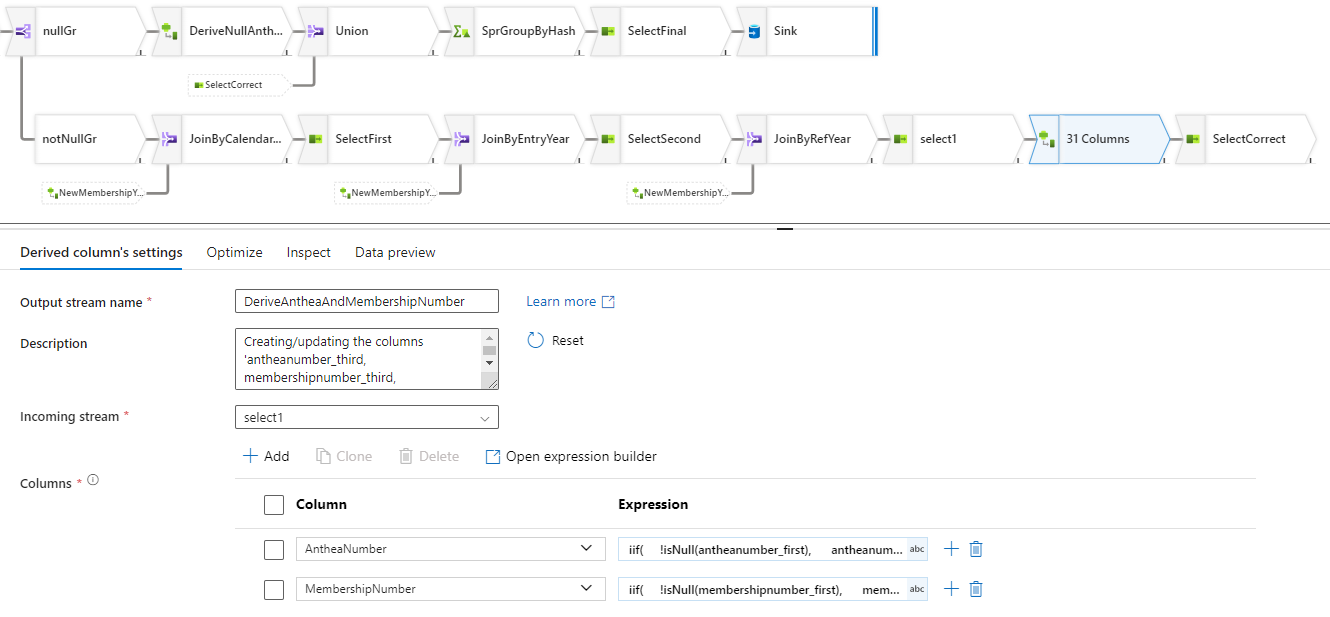
\includegraphics[width=0.9\textwidth]{./graphics/adf/member_7.png}
    \footnote{Derive van kolommen `AntheaNumber` en `MembershipNumber` op de tabel `new\_syndicalpremiumrequest`}
\end{center}

De kolommen `AntheaNumber` en `MembershipNumber` worden nu berekent.

\begin{minted}{text}
iif(!isNull(antheanumber_first), antheanumber_first,      
    iif(!isNull(antheanumber_second), antheanumber_second,
        iif(!isNull(antheanumber_third), antheanumber_third, toString(null()))))
\end{minted}

Wanneer het antheanummer van de eerste join niet NULL is zal deze gebruikt worden, anders zal er gekeken worden of de tweede niet NULL is. Als de tweede NULL is zal de derde gebruikt worden. Indien de derde ook NULL is zal dit resulteren in NULL als waarde voor de kolom `AntheaNumber`.

\begin{minted}{text}
iif(!isNull(membershipnumber_first), membershipnumber_first, 
    iif(!isNull(membershipnumber_second), membershipnumber_second,         
        iif(!isNull(membershipnumber_third), membershipnumber_third, toString(null()))))
\end{minted}

Ook de kolom `MembershipNumber` wordt op dezelfde manier berekent.

\begin{center}
    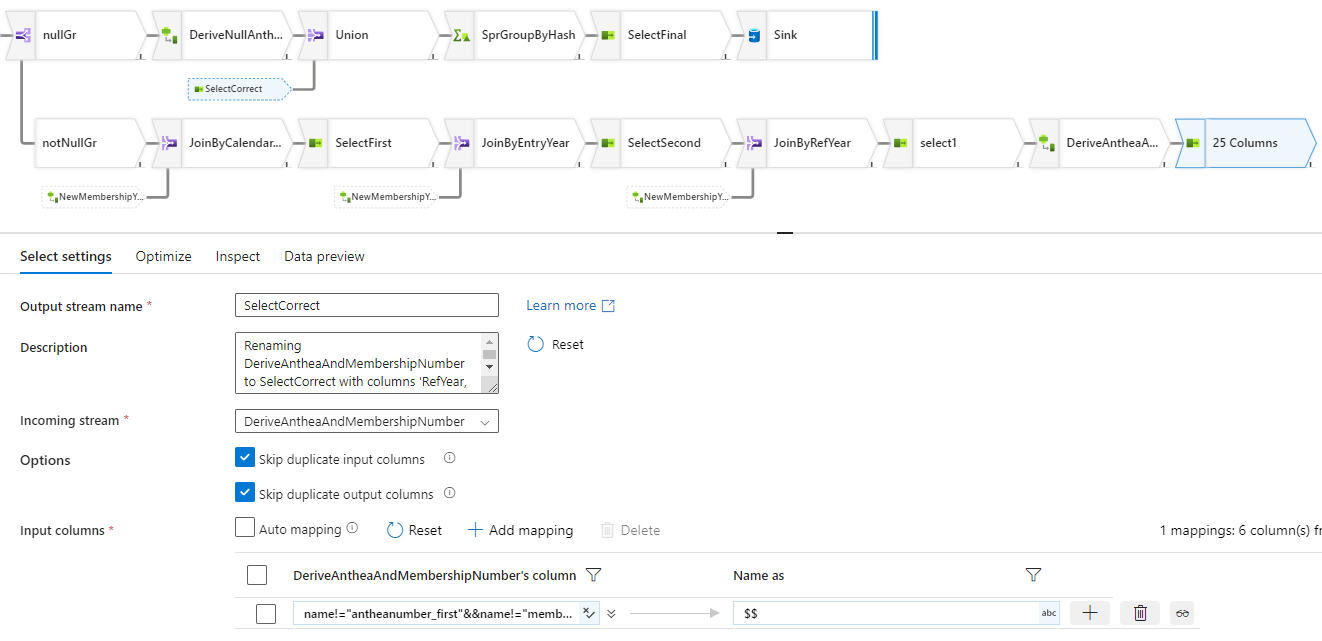
\includegraphics[width=0.9\textwidth]{./graphics/adf/member_8.png}
    \footnote{Verwijderen van onnodige kolommen op de tabel `new\_syndicalpremiumrequest`}
\end{center}

De kolommen die niet nodig zijn worden verwijderd.

\begin{center}
    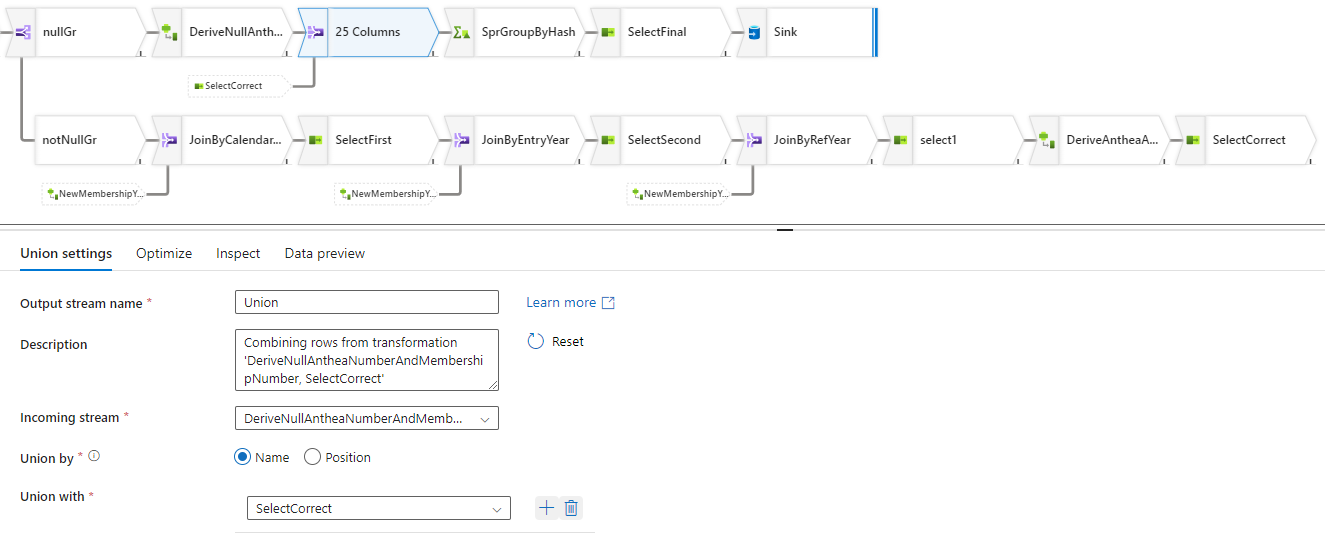
\includegraphics[width=0.9\textwidth]{./graphics/adf/member_9.png}
    \footnote{Union van twee streams}
\end{center}

Beide streams worden nu samen gevoegd met behulp van een union.

En ten slotte is het ook voor deze transformatie belangrijk dat er geaggregeerd wordt zoals bij Figuur \ref{fig:groupby} om te voorkomen dat dezelfde premie twee keer in een groep voor een bepaald jaartal terecht komt.

\subsection{Azure Databricks}

\subsubsection{Opzet van resources}

\begin{center}
    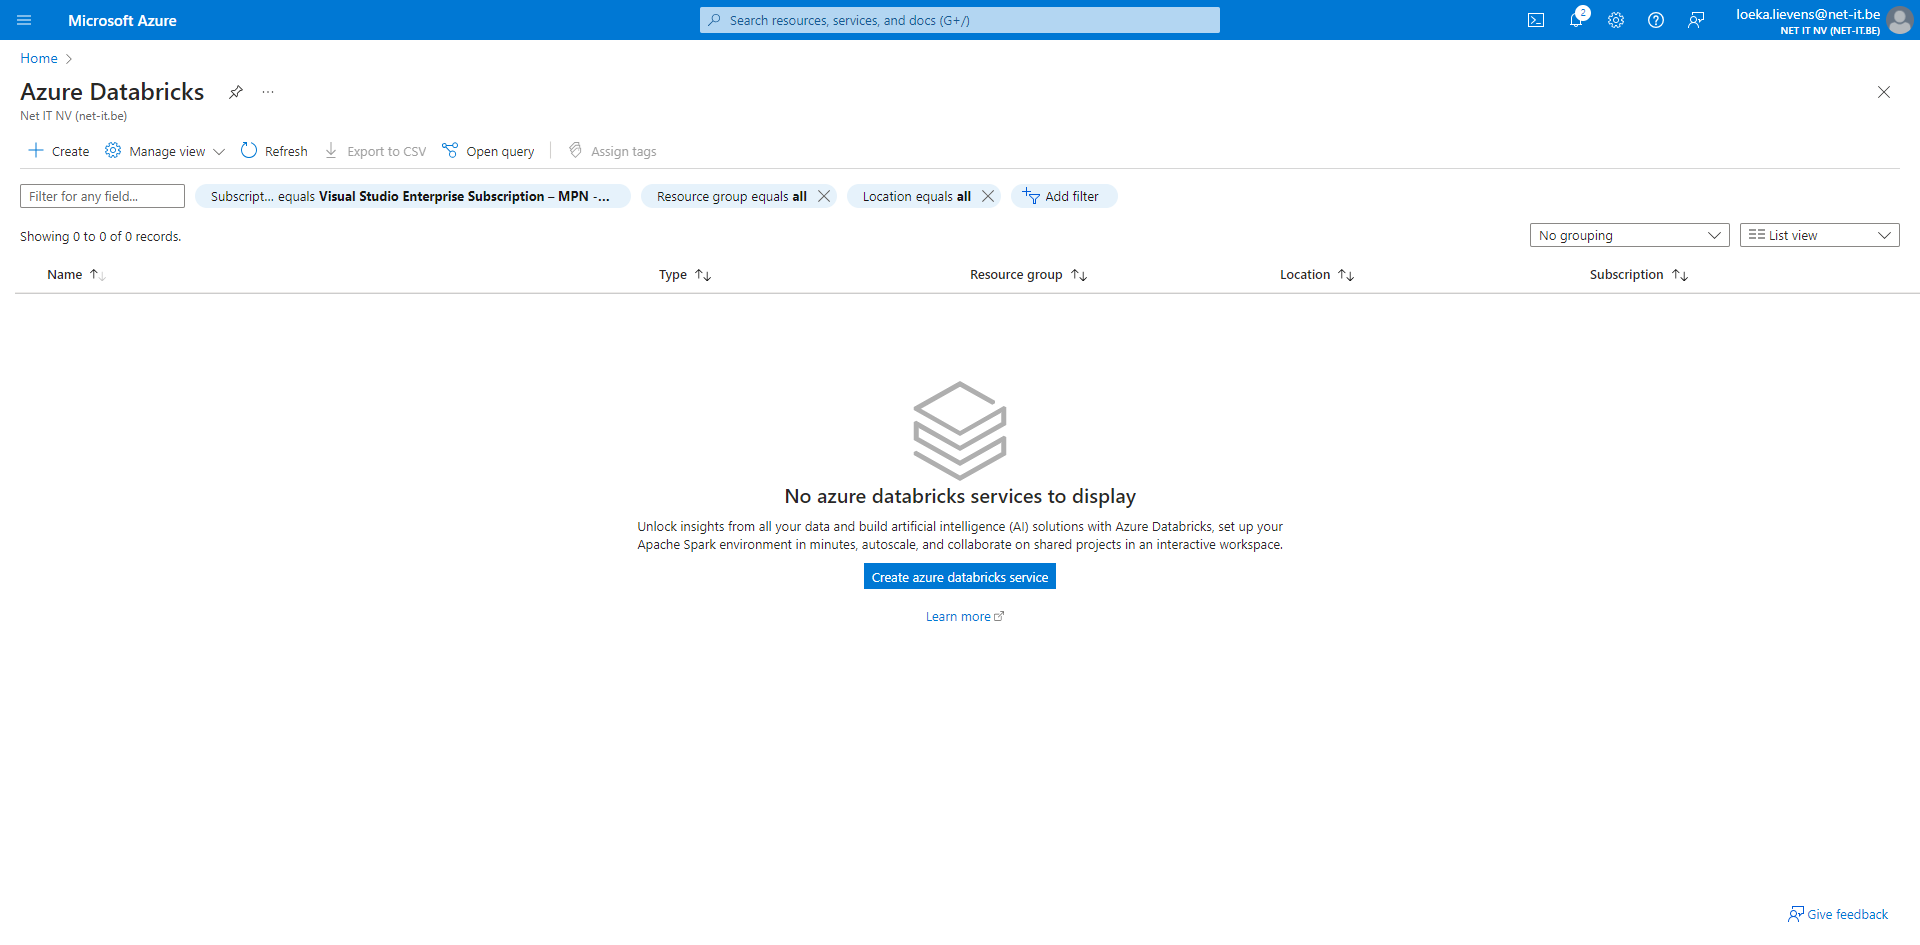
\includegraphics[width=0.9\textwidth]{./graphics/databricks/initial_1.png}
    \footnote{Aanmaken van Azure Databricks}
\end{center}

Door in Microsoft Azure naar Databricks te navigeren kunnen we een nieuwe Azure Databricks workspace gaan aanmaken.

\begin{center}
    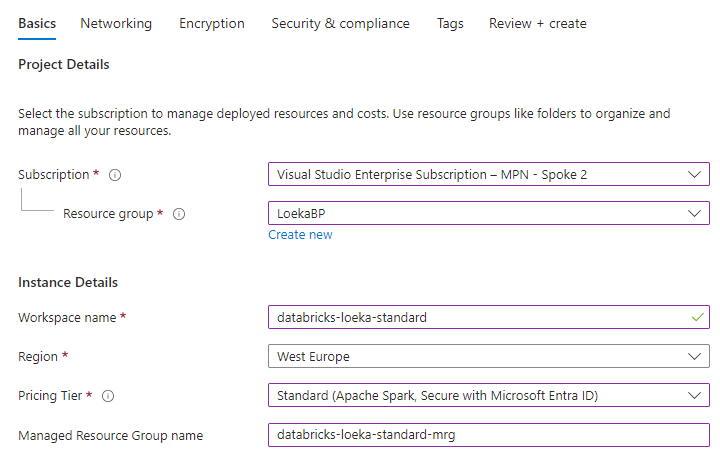
\includegraphics[width=0.6\textwidth]{./graphics/databricks/initial_2.png}
    \footnote{Configuratie van Azure Databricks}
\end{center}

Bij het aanmaken van databricks moet er een subscription en resource group gekozen worden. Er kan een nieuwe resource group aangemaakt worden of een reeds bestaande gekozen worden. Daarnaast moet er een naam, gewenste regio en pricing tier gekozen worden. Als pricing tier kiezen we hier voor Standard doordat we geen gebruik gaan maken van Premium features. Ten slotte kan er ook een Managed Resource Group name gekozen worden. Deze resource group houdt alle resource bij die databricks nodig heeft, zoals bijvoorbeeld virtual machines, storage accounts en virtual networks.

\begin{center}
    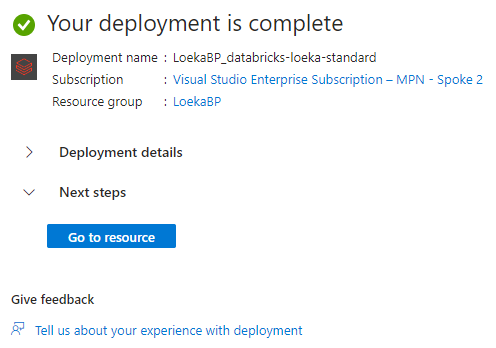
\includegraphics[width=0.6\textwidth]{./graphics/databricks/initial_3.png}
    \footnote{Deployment complete van Azure Databricks}
\end{center}

Wanneer de resource is aangemaakt kan Azure Databricks opgestart worden.

\begin{center}
    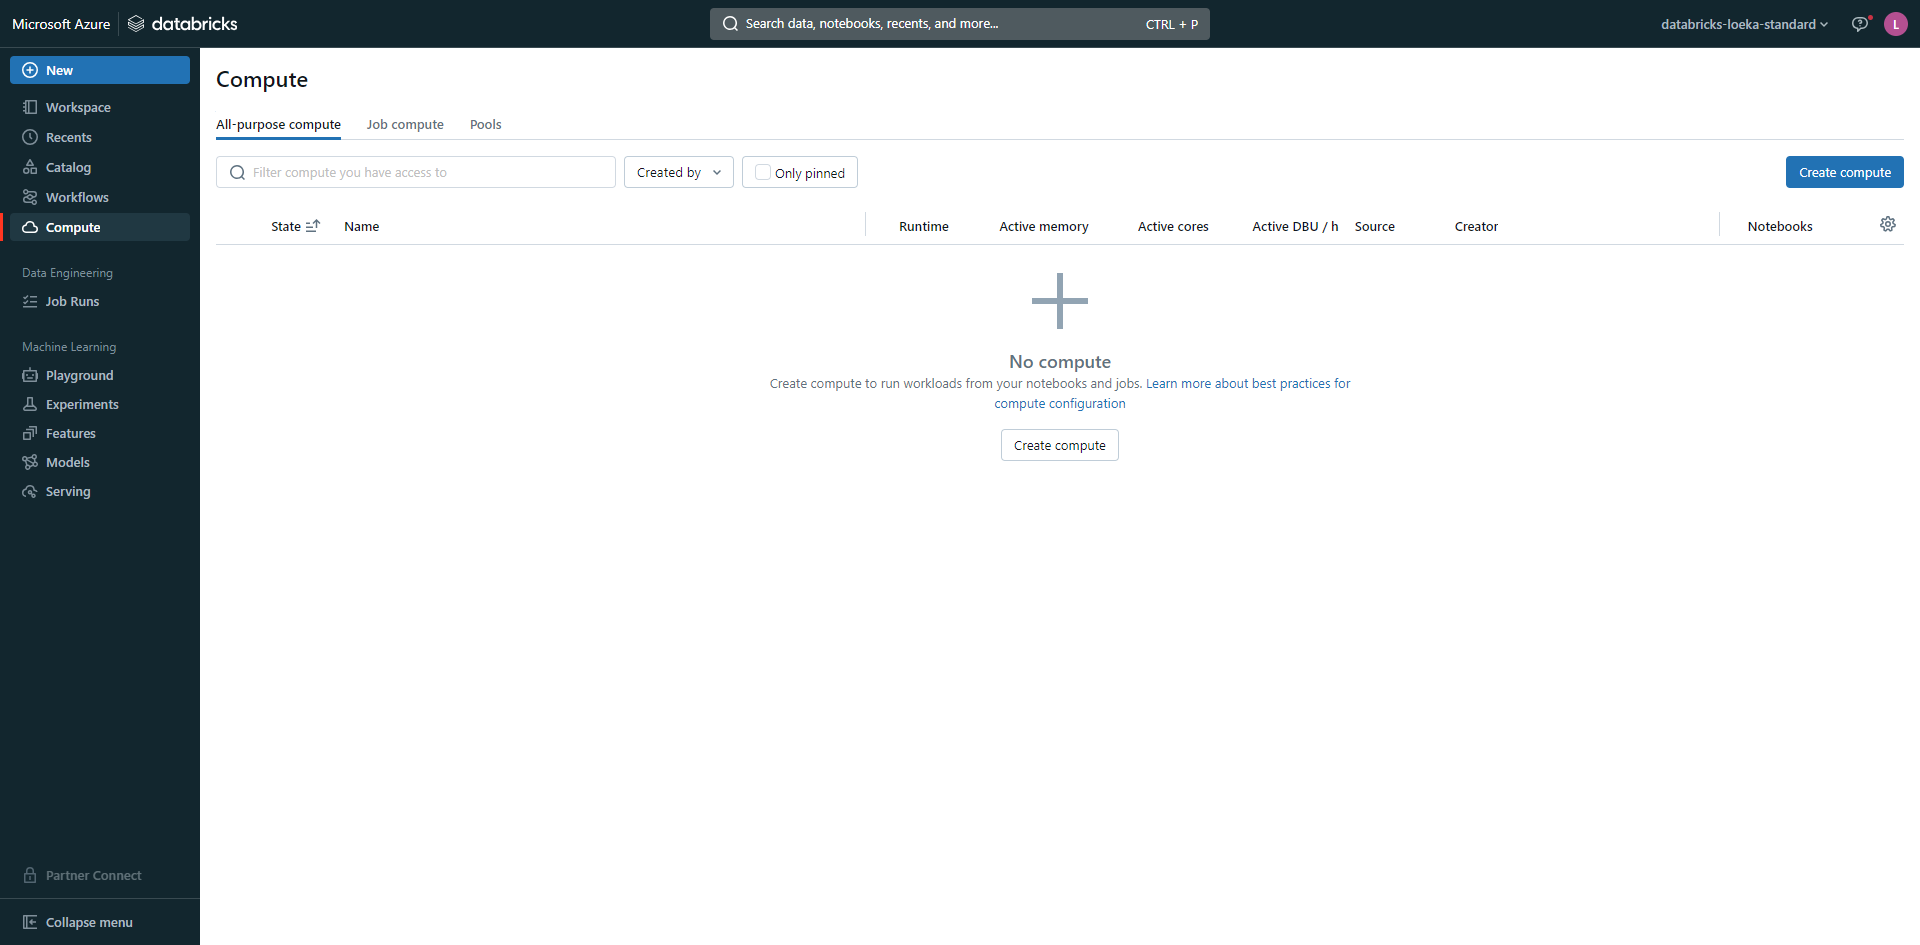
\includegraphics[width=0.9\textwidth]{./graphics/databricks/initial_4.png}
    \footnote{Aanmaken van compute resource}
\end{center}

Voor we notebooks en jobs gaan kunnen uitvoeren zullen we eerst een compute resource moeten gaan aanmaken.

\begin{center}
    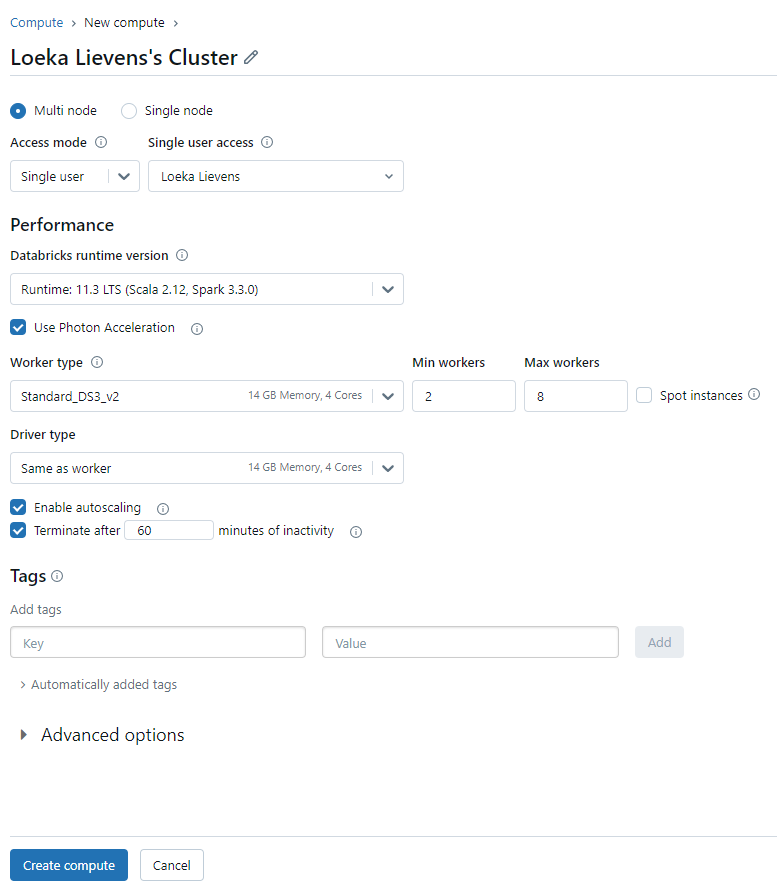
\includegraphics[width=0.6\textwidth]{./graphics/databricks/initial_5.png}
    \footnote{Configuratie van compute resource}
\end{center}

De databricks runtime version moet op 11.3 LTS gezet worden zodat we Apache Spark 3.3.0 kunnen gebruiken. Dit omdat we gebruik gaan maken van `spark-cdm-connector`. Ook hebben we ingesteld dat de cluster zichzelf zal uitschakelen na 60 minuten om onnodige kosten te voorkomen.

\begin{center}
    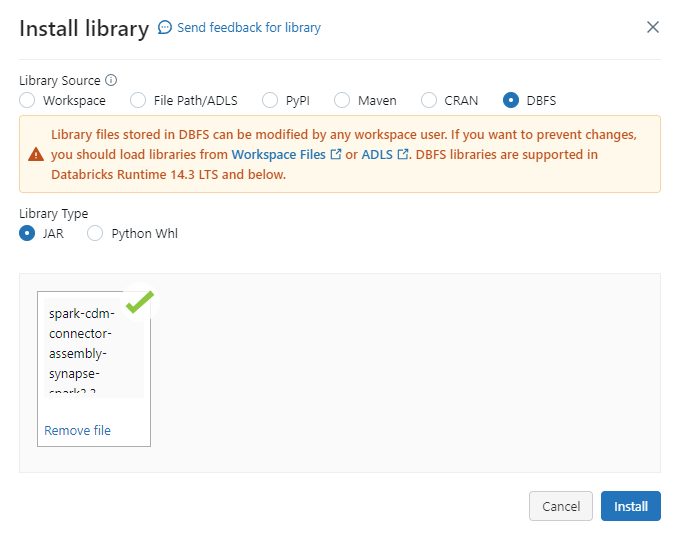
\includegraphics[width=0.9\textwidth]{./graphics/databricks/initial_6.png}
    \footnote{Installatie van `spark-cdm-connector`}
\end{center}

Ten slotte moet de \href{https://github.com/Azure/spark-cdm-connector/releases/tag/spark3.3-1.19.5}{jar file} van `spark-cdm-connector` geïnstalleerd worden in het aangemaakte compute resource om gebruik te kunnen maken van het Common Data Model in onze pipeline.

\subsubsection{Collaboration en source control}

\textbf{Management en permissions}

\begin{center}
    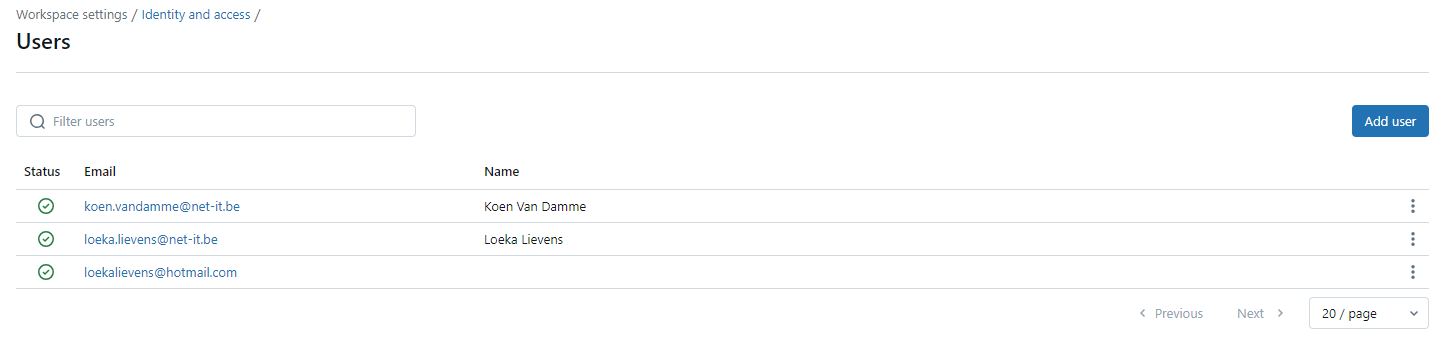
\includegraphics[width=0.9\textwidth]{./graphics/databricks/management_permissions_1.png}
    \footnote{Gebruikers toevoegen/verwijderen in Azure Databricks}
\end{center}

Gebruikers die behoren tot het AAD directory van de Azure Databricks environment kunnen makkelijk toegevoegd worden met behulp van het e-mailadres van de gebruiker.

\begin{center}
    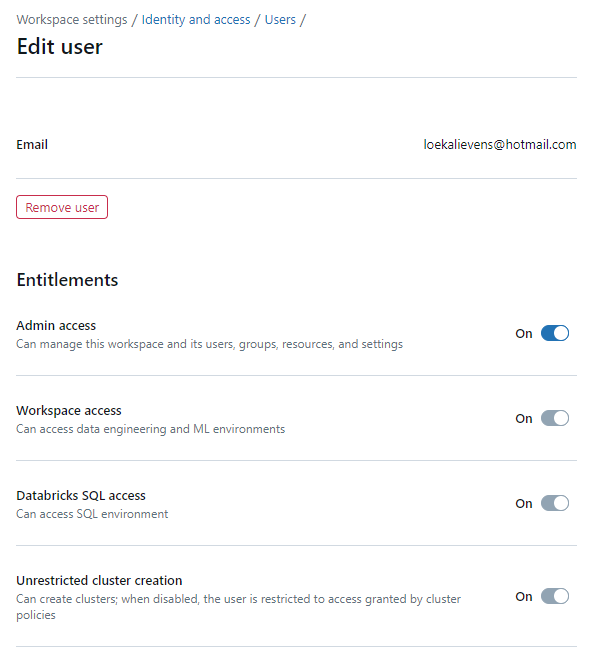
\includegraphics[width=0.6\textwidth]{./graphics/databricks/management_permissions_2.png}
    \footnote{Rechten wijzigen van gebruikers in Azure Databricks}
\end{center}

Rechten van gebruikers kunnen gewijzigd worden.

\begin{center}
    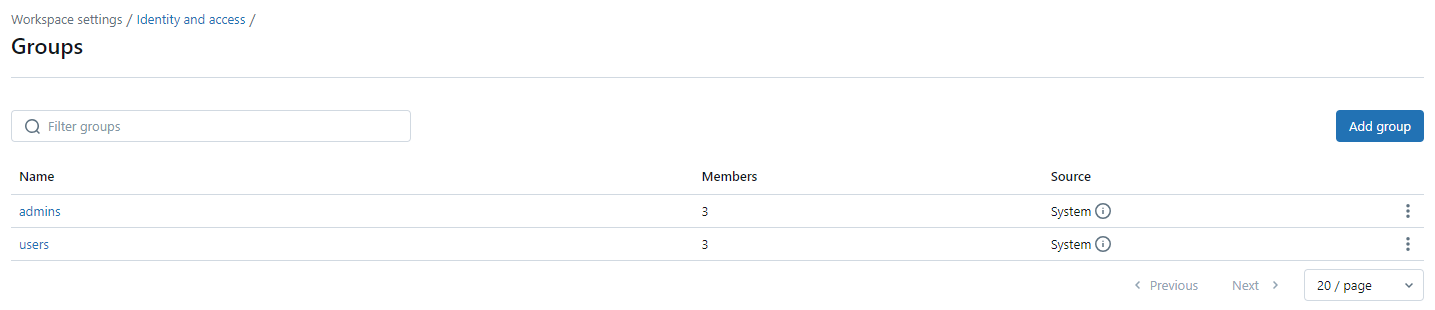
\includegraphics[width=0.9\textwidth]{./graphics/databricks/management_permissions_3.png}
    \footnote{Groepen toevoegen of verwijderen in Azure Databricks}
\end{center}

Er kunnen groepen toegevoegd of verwijderd worden aan Azure Databricks. Gebruikers kunnen dan aan deze groepen toegevoegd worden. Dit vereenvoudigt het om toegang toe te wijzen aan werkruimten, gegevens en andere objecten.

\textbf{Source control}

Databricks folders is een visuele Git client binnen Azure Databricks om gebruik te kunnen maken van source control.

\begin{center}
    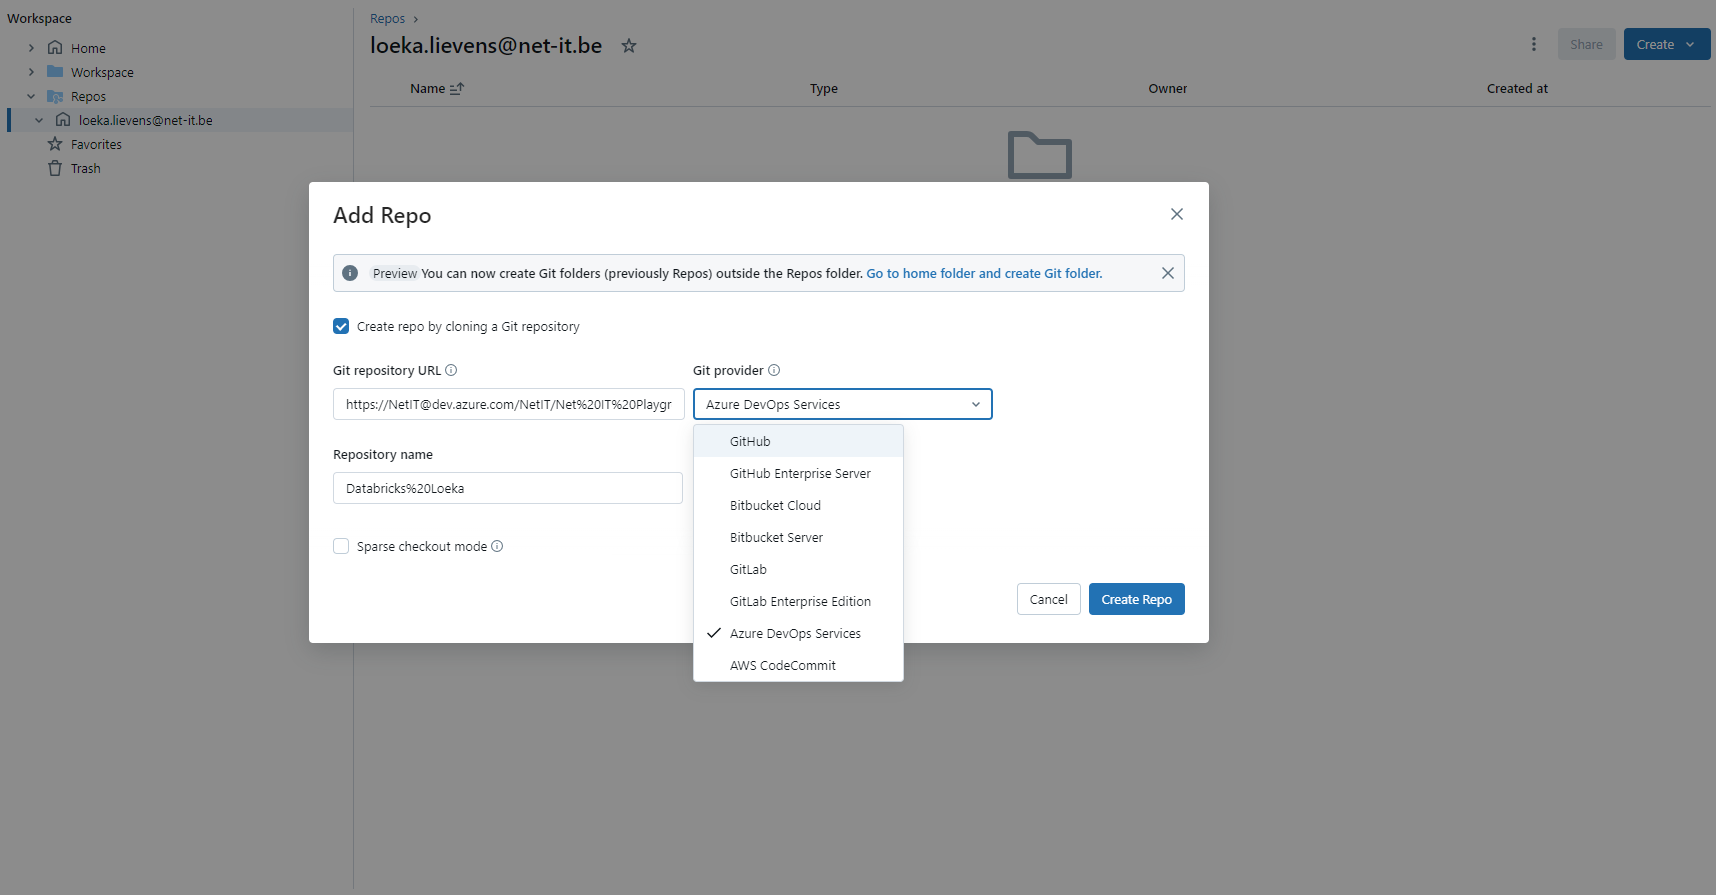
\includegraphics[width=0.9\textwidth]{./graphics/databricks/git_1.png}
    \footnote{Clone Git repository in Databricks folders}
\end{center}

Het geeft de optie om verschillende Git providers te gaan gebruiken. Doordat er binnen Net IT gewerkt wordt met Azure DevOps Services zal hier voor gekozen worden.

\begin{center}
    \includegraphics[width=0.9\textwidth]{./graphics/databricks/git_2.png}
    \footnote{Aanmaken van een notebook in databricks}
\end{center}

Ter illustratie zal er een voorbeeld notebook aangemaakt worden.

\begin{center}
    \includegraphics[width=0.9\textwidth]{./graphics/databricks/git_3.png}
    \footnote{Commit en push in Databricks}
\end{center}

\begin{center}
    \includegraphics[width=0.9\textwidth]{./graphics/databricks/git_4.png}
    \footnote{Commit en push in Databricks}
\end{center}

Deze notebook kan dan gecommit worden naar Git.

\subsubsection{Ophalen van data uit Azure Data Lake}

\begin{center}
    \includegraphics[width=0.9\textwidth]{./graphics/databricks/connection_1.png}
    \footnote{App registration aanmaken}
\end{center}

\begin{center}
    \includegraphics[width=0.9\textwidth]{./graphics/databricks/connection_2.png}
    \footnote{Configuratie app registration}
\end{center}

Door in Microsoft Azure naar `App registrations` te navigeren kunnen we een nieuwe app registration aanmaken.

\begin{center}
    \includegraphics[width=0.9\textwidth]{./graphics/databricks/connection_3.png}
    \footnote{Aanmaken client secret}
\end{center}

Door naar `Certificates \& secrets` in de app registration te navigeren kunnen we een client secret gaan aanmaken. Het is belangrijk om deze client secret op te slaan.

\begin{center}
    \includegraphics[width=0.9\textwidth]{./graphics/databricks/connection_4.png}
    \footnote{Role assignment toevoegen aan storage account}
\end{center}

Wanneer we nu naar `Access Control (IAM)` navigeren van het storage account waarmee we een connectie willen maken kunnen we nu een role assignment gaan toevoegen.

\begin{center}
    \includegraphics[width=0.9\textwidth]{./graphics/databricks/connection_5.png}
    \footnote{Job function role kiezen voor role assignment}
\end{center}

Als job function role kiezen we voor `Storage Blob Data Contributor`.

\begin{center}
    \includegraphics[width=0.9\textwidth]{./graphics/databricks/connection_6.png}
    \footnote{Members kiezen voor role assignment}
\end{center}

Bij `Members` kiezen we voor de service principal die we net hebben aangemaakt.

\begin{center}
    \includegraphics[width=0.9\textwidth]{./graphics/databricks/connection_7.png}
    \footnote{Key vault aanmaken}
\end{center}

Door in Microsoft Azure naar `Key vaults` te navigeren kunnen we een nieuwe key vault gaan aanmaken.

\begin{center}
    \includegraphics[width=0.9\textwidth]{./graphics/databricks/connection_8.png}
    \footnote{Configuratie van key vault}
\end{center}

Bij het aanmaken van een key vault moet er een subscription en resource group gekozen worden. Er kan een nieuwe resource group aangemaakt worden of een reeds bestaande gekozen worden. Daarnaast moet er een naam, gewenste regio en pricing tier gekozen worden.

\begin{center}
    \includegraphics[width=0.9\textwidth]{./graphics/databricks/connection_9.png}
    \footnote{Permission model van key vault}
\end{center}

Onder `Access configuration` kiezen we voor `Vault access policy` als permission model.

\begin{center}
    \includegraphics[width=0.9\textwidth]{./graphics/databricks/connection_10.png}
    \footnote{Networking configuratie van key vault}
\end{center}

Er kan gekozen worden om enkel geselecteerde networks public access te geven of om public access uit te schakelen. Belangrijk is dat `Allow trusted Microsoft services to bypass this firewall` aangevinkt staat.

\begin{center}
    \includegraphics[width=0.9\textwidth]{./graphics/databricks/connection_11.png}
    \footnote{Deployment complete van key vault}
\end{center}

Wanneer onze resource aangemaakt is kunnen we naar de key vault navigeren.

\begin{center}
    \includegraphics[width=0.9\textwidth]{./graphics/databricks/connection_12.png}
    \footnote{Toevoegen van een secret in key vault}
\end{center}

Door naar `Secrets` te navigeren in de key vault kunnen we nu onze client secret toevoegen.

\begin{center}
    \includegraphics[width=0.9\textwidth]{./graphics/databricks/connection_13.png}
    \footnote{Opzoeken van properties van key vault}
\end{center}

Door naar `Properties` te navigeren kunnen we nu `Vault URI` en `Resource ID` vinden. Deze zijn belangrijk voor de volgende stap.

\begin{center}
    \includegraphics[width=0.9\textwidth]{./graphics/databricks/connection_14.png}
    \footnote{Aanmaken van secret scope in databricks}
\end{center}

Door naar `https://<databricks-instance>\#secrets/createScope` te navigeren kunnen we nu een secret scope aanmaken in databricks. Hiervoor hebben we `Vault URI` en `Resource ID` nodig uit de vorige stap.

\begin{center}
    \includegraphics[width=0.9\textwidth]{./graphics/databricks/connection_15.png}
    \footnote{Ophalen van secrets uit key vault}
\end{center}

We kunnen nu in onze notebooks met bovenstaande code secrets zoals bijvoorbeeld `AppKey` ophalen uit key vault.

%\begin{center}
%    \includegraphics[width=0.9\textwidth]{./graphics/databricks/connection_16.png}
%    \footnote{Configuratie van `spark-cdm-connector`}
%\end{center}

\begin{minted}{python}
storage_account = "<storage-account>"
app_id = "<application-id>"
app_key = dbutils.secrets.get(scope = "KeyVault", key = "AppKey")
tenant_id = "<directory-id>"
\end{minted}

Om een connectie te kunnen maken met data lake hebben we `storage\_account`, `app\_id`, `app\_key` en `tenant\_id` nodig. Dit kunnen we doen door het volgende te vervangen:

\begin{itemize}
    \item `<storage-account>` met de naam van het Azure storage account
    \item `<application-id>` met het Application (client) ID voor de Microsoft Entra ID application
    \item `<directory-id>` met het Directory (tenant) ID voor de Microsoft Entra ID application
\end{itemize}

%\begin{center}
%    \includegraphics[width=0.9\textwidth]{./graphics/databricks/connection_17.png}
%    \footnote{Configuratie van `spark-cdm-connector`}
%\end{center}

\begin{minted}{python}
df = spark.read.format("com.microsoft.cdm") \
    .option("appId", app_id) \
    .option("appKey", app_key) \
    .option("tenantId", tenant_id) \
    .option("storage", f"{storage_account}.dfs.core.windows.net") \
    .option("manifestPath", "sourcedata/model.json") \
    .option("mode", "permissive")
\end{minted}

We kunnen nu gebruik maken van `spark-cdm-connector` door `com.microsoft.cdm` mee te geven. Het is belangrijk dat `mode` op `permissive` staat, dit zorgt er voor dat er null values assigned worden wanneer een CSV rij minder aantal kolommen heeft dan het entity schema.

%\begin{center}
%    \includegraphics[width=0.9\textwidth]{./graphics/databricks/connection_18.png}
%    \footnote{Laden van de nodige entiteiten in databricks}
%\end{center}

\begin{minted}{python}
spr = df.option("entity", "new_syndicalpremiumrequest") \
    .load()
\end{minted}

Met bovenstaande code kan een entiteit ingeladen worden in een variabele. Dit zal dus ook gebeuren met alle entiteiten die we hebben.

%\begin{center}
%    \includegraphics[width=0.9\textwidth]{./graphics/databricks/connection_19.png}
%    \footnote{Selecteren van kolommen en aanmaken van temporary views in databricks}
%\end{center}

\begin{minted}{python}
spr \
    .select("Id", "new_personid", "new_bankaccountid", "new_scannedrequestcode", "new_isdeclarationonhonour", "new_requesttypeid", "new_formnumber", "new_treatmentstate", "new_feedback", "new_reasonforcontrol", "new_yearid", "createdon", "new_idadm", "new_contributionamount", "new_premiumamount", "new_paymentdate", "new_remarkgroupfinal", "new_groupid") \
    .createOrReplaceTempView("new_syndicalpremiumrequest")
\end{minted}

Voor elke entiteit die we hebben ingeladen in een variabele zullen we nu de nodige kolommen gaan selecteren. Hierna kan er een temporary view aangemaakt worden voor de entiteiten. Daardoor kunnen we later queries gaan uitvoeren in SQL om zo transformaties uit te voeren.

\subsubsection{Belangrijkste transformaties}

\textbf{Determinatie van welke groepen de premie in hun bestand krijgen}

\begin{minted}[highlightlines={4, 5, 6, 56}]{sql}
CREATE
OR REPLACE TEMPORARY VIEW spr_stage_1 AS
SELECT 
    YEAR(spr.createdon) EntryYear, 
    YEAR(GETDATE()) CalendarYear, 
    CAST(ny.new_year AS INTEGER) RefYear, 
    IF(spr.new_scannedrequestcode == 552010000, IF(spr.new_isdeclarationonhonour, "DOH", "FORM"), IF(spr.new_scannedrequestcode == 552010001, "QR", "UNKNOWN")) Type,
    
    IF(spr.new_requesttypeid == "d026f6f9-fc82-ea11-a811-000d3a2d0171", CONCAT(SUBSTRING(new_formnumber, 1, 4), "-", SUBSTRING(new_formnumber, 5, 6), "-", SUBSTRING(new_formnumber, 11, 20)), spr.new_formnumber) Form,
    
    IF(rpr.new_treatmentstate == 552010004,
        CASE
            WHEN spr.new_treatmentstate == 552010000 THEN "1"
            WHEN spr.new_treatmentstate == 552010001 THEN "10"
            WHEN spr.new_treatmentstate == 552010002 THEN "1"
            WHEN spr.new_treatmentstate == 552010003 THEN "10"
            WHEN spr.new_treatmentstate == 552010004 THEN "5"
            WHEN spr.new_treatmentstate == 552010005 THEN "11"
            WHEN spr.new_treatmentstate == 552010006 THEN "1"
            WHEN spr.new_treatmentstate == 552010007 THEN "10"
            WHEN spr.new_treatmentstate == 552010008 THEN "8"
            ELSE ""
        END,
        CASE
            WHEN spr.new_treatmentstate == 552010000 THEN "1"
            WHEN spr.new_treatmentstate == 552010001 THEN "2"
            WHEN spr.new_treatmentstate == 552010002 THEN "1"
            WHEN spr.new_treatmentstate == 552010003 THEN "2"
            WHEN spr.new_treatmentstate == 552010004 THEN "5"
            WHEN spr.new_treatmentstate == 552010005 THEN "11"
            WHEN spr.new_treatmentstate == 552010006 THEN "1"
            WHEN spr.new_treatmentstate == 552010007 THEN "2"
            WHEN spr.new_treatmentstate == 552010008 THEN "8"
            ELSE ""
        END
    ) Status,
    IF(spr.new_feedback, "FEEDBACK", spr.new_reasonforcontrol) AvalonRemark,
    
    spr.new_personid,
    spr.new_idadm,
    spr.new_yearid,
    spr.id,
    spr.createdon,
    spr.new_contributionamount,
    spr.new_premiumamount,
    spr.new_paymentdate,
    ba.new_bankaccount,
    spr.new_remarkgroupfinal,
    p.new_firstname,
    p.new_lastname,
    p.new_dateofbirth
FROM new_syndicalpremiumrequest spr
LEFT JOIN new_person p ON spr.new_personid = p.new_personid
LEFT JOIN new_bankaccount ba ON spr.new_bankaccountid = ba.new_bankaccountid
LEFT JOIN related_premium_requests rpr ON spr.Id = rpr.new_syndicalpremiumrequestid
LEFT JOIN new_year ny ON spr.new_yearid = ny.new_yearid;
\end{minted}

De tabel `new\_year` wordt opnieuw gejoind op de tabel `new\_syndicalpremiumrequest` met behulp van de kolom `new\_yearid`. Daarnaast wordt ook hier de drie kolommen EntryYear, CalendarYear en RefYear berekent. Deze worden op dezelfde manier berekent als bij de transformatie in Azure Data Factory.


\begin{minted}{sql}
CREATE
OR REPLACE TEMPORARY VIEW spr_stage_2 AS
SELECT 
    explode(array(nm.new_groupid, noy.new_groupid)) new_groupid,
    spr.*,
    nm.new_groupprefix new_groupprefix
FROM spr_stage_1 spr
LEFT JOIN new_membership_stage_1 nm 
    ON (spr.CalendarYear = nm.new_year OR spr.EntryYear = nm.new_year OR RefYear == nm.new_year) AND spr.new_personid == nm.new_personid 
LEFT JOIN new_organizationyear_stage_1 noy 
    ON spr.new_idadm == noy.new_idadmaux AND spr.new_yearid == noy.new_yearid;
\end{minted}

De tabellen `new\_membership` en `new\_organizationyear` worden gejoind op de tabel `new\_syndicalpremiumrequest` om de groepen te gaan bepalen. Zoals te zien in de code snippet hierboven noemen deze tabellen `new\_membership\_stage\_1` en `new\_organizationyear\_stage\_1`. Dit komt doordat er reeds andere transformaties zijn geweest.

Bij de tabel `new\_membership` wordt er, net zoals in Azure Data Factory, gekeken of CalendarYear, EntryYear of RefYear overeenkomt met het jaartal van de membership. Daarnaast wordt er ook gekeken of personid overeen komt. 

Bij de tabel `new\_organizationyear` wordt er gejoind met behulp van IDADM en het id van het referentiejaar.

\begin{center}%
    \begin{tabularx}{0.7\textwidth}{ |X|X|X| }
        \hline
        spr.Id & nm.new\_groupid & noy.new\_groupid \\
        \hline 
        101e4523-7c60-45ff-a928-087ca139d8f5  & 2ad31fb8-5117-4627-a2a3-a5fdbee5b9ae & null  \\
        \hline
        f5ac28c0-6b80-412a-b0e6-f9a82feff9a1 & f1015dd0-3096-478d-ae12-4226c101dd54 & a2974e74-be93-4326-9d18-f4bb2abc0842 \\
        \hline
    \end{tabularx}
    
    \Bigg\downarrow

    \begin{tabularx}{0.7\textwidth}{ |X|X| }
        \hline
        spr.Id & new\_groupid \\
        \hline 
        101e4523-7c60-45ff-a928-087ca139d8f5  & 2ad31fb8-5117-4627-a2a3-a5fdbee5b9ae  \\
        \hline
        101e4523-7c60-45ff-a928-087ca139d8f5  & null  \\
        \hline
        f5ac28c0-6b80-412a-b0e6-f9a82feff9a1 & f1015dd0-3096-478d-ae12-4226c101dd54 \\
        \hline
        f5ac28c0-6b80-412a-b0e6-f9a82feff9a1 & a2974e74-be93-4326-9d18-f4bb2abc0842 \\
        \hline
    \end{tabularx}
\end{center}

Deze twee joins resulteren in twee nieuwe kolommen `nm.new\_groupid` en `noy.new\_groupid`. Met behulp van de `explode` functie zorgen we er voor dat deze twee kolommen één kolom zullen worden. Één rij zal dan bijvoorbeeld twee rijen worden. Deze twee rijen zijn dan volledig hetzelfde met het verschil dat de kolom `new\_groupid` voor de eerste rij de waarde van `nm.new\_groupid` heeft en voor de tweede rij de waarde van `noy.new\_groupid`.


\begin{minted}{sql}
CREATE 
OR REPLACE TEMPORARY VIEW spr_stage_3 AS 
SELECT 
    FIRST(id) id, 
    FIRST(new_groupid) new_groupid, 
    FIRST(new_personid) new_personid,
    FIRST(CalendarYear) CalendarYear,
    FIRST(EntryYear) EntryYear,
    FIRST(RefYear) RefYear,
    FIRST(new_groupprefix) new_groupprefix,
    FIRST(createdon) createdon,
    FIRST(new_contributionamount) new_contributionamount,
    FIRST(new_premiumamount) new_premiumamount,
    FIRST(new_paymentdate) new_paymentdate,
    FIRST(new_bankaccount) new_bankaccount,
    FIRST(new_remarkgroupfinal) new_remarkgroupfinal,
    FIRST(AvalonRemark) AvalonRemark,
    FIRST(new_firstname) new_firstname,
    FIRST(new_lastname) new_lastname,
    FIRST(new_dateofbirth) new_dateofbirth,
    FIRST(Type) Type,
    FIRST(Form) Form,
    FIRST(Status) Status,
    FIRST(new_idadm) new_idadm
FROM spr_stage_2 
WHERE id IS NOT NULL AND new_groupid IS NOT NULL AND RefYear IS NOT NULL
GROUP BY (id, new_groupid, RefYear);
\end{minted}

Ten slotte gaan we een `GROUP BY` clause gebruiken om er voor te zorgen dat een premie niet twee keer naar dezelfde groep voor dat referentiejaar wordt gestuurd. Daarnaast wordt er ook gefilterd zodat er geen premies zijn zonder id, groupid of referentiejaar. Met behulp van de `FIRST` aggregrate function selecteren we steeds de eerste waarde voor de nodige kolommen. We hebben nu een tabel met alle premies waarvan we weten naar welke groep voor welk referentiejaar ze gestuurd moeten worden.

\textbf{Bepalen van de kolom `Gr` voor een premie}

\begin{minted}[highlightlines={4}]{sql}
CREATE
OR REPLACE TEMPORARY VIEW nm_grouped_by AS
SELECT 
    FIRST(new_groupprefix, TRUE) new_groupprefix, 
    FIRST(new_personid) new_personid, 
    FIRST(new_year) new_year 
FROM new_membership_stage_1
WHERE new_groupprefix IS NOT NULL 
GROUP BY (new_personid, new_year);

CREATE 
OR REPLACE TEMPORARY VIEW spr_stage_4 AS 
SELECT
spr.*,
    CASE
        WHEN spr.new_groupprefix IS NOT NULL THEN spr.new_groupprefix
        WHEN nmCalendar.new_groupprefix IS NOT NULL THEN nmCalendar.new_groupprefix
        WHEN nmEntry.new_groupprefix IS NOT NULL THEN nmEntry.new_groupprefix
        WHEN nmRef.new_groupprefix IS NOT NULL THEN nmRef.new_groupprefix
        ELSE NULL
    END Gr
FROM spr_stage_3 spr
LEFT JOIN nm_grouped_by nmCalendar ON spr.new_personid = nmCalendar.new_personid AND spr.CalendarYear = nmCalendar.new_year
LEFT JOIN nm_grouped_by nmEntry ON spr.new_personid = nmEntry.new_personid AND spr.EntryYear = nmEntry.new_year
LEFT JOIN nm_grouped_by nmRef ON spr.new_personid = nmRef.new_personid AND spr.RefYear = nmRef.new_year;
\end{minted}

Voor het bepalen van de kolom `Gr` in databricks wordt er eerst een temporary view `nm\_grouped\_by` aangemaakt waarbij er gegroepeerd wordt op `new\_personid` en `new\_year`. Dit zal er voor zorgen dat de joins die we uitvoeren zullen resulteren in één enkele match (of geen). De tweede parameter in de functie `FIRST` (aangeduid in code snippet) zorgt er voor dat NULL values genegeerd worden. De eeste waarde die niet NULL is voor `new\_groupprefix` zal dus geselecteerd worden.

De temporary view die we hebben aangemaakt wordt nu drie keer gejoind op de tabel `spr\_stage\_3` aan de hand van `new\_personid` en CalendarYear, EntryYear of RefYear. `Gr` zal bepaald worden door eerst te kijken of `spr.new\_groupprefix` niet NULL is, wanneer deze wel NULL is zal er gekeken worden naar `nmCalendar.new\_groupprefix`, `nmEntry.new\_groupprefix` en ten slotte naar `nmRef.new\_groupprefix`.

% Einde nieuw

%\begin{center}
%    \includegraphics[width=1\textwidth]{./graphics/adf/initial_1.png}
%\end{center}
%
%Selecteer een gewenste subsscription en resource group. Er kan gekozen worden voor een resource group die er al bestaat of om een nieuwe aan te maken. Hier na kan er een naam en gewenste regio gekozen worden. De version laten we staan op V2.
%
%\begin{center}
%    \includegraphics[width=1\textwidth]{./graphics/adf/initial_2.png}
%\end{center}
%
%Door bij de vorige stap op next te klikken kunnen we er voor kiezen om een Git configuratie te gaan toevoegen. Dit zullen we pas later gaan doen. Klik nu op `Review + create` om de data factory aan te maken.
%
%\begin{center}
%    \includegraphics[width=1\textwidth]{./graphics/adf/deployment_complete.png}
%\end{center}
%
%Wanneer onze deployment complete is kunnen we naar onze resource gaan door op `Go to resource` te klikken.
%
%\begin{center}
%    \includegraphics[width=1\textwidth]{./graphics/adf/launch_adf.png}
%\end{center}
%
%Klik nu op `Launch studio` om naar Azure Data Factory Studio te gaan.
%
%\subsubsection{Koppeling met Git}
%
%\begin{center}
%    \includegraphics[width=1\textwidth]{./graphics/adf/setup_repository.png}
%\end{center}
%
%Voor we onze ETL gaan implementeren zullen we eerst onze data factory koppelen met Git.
%
%\begin{center}
%    \includegraphics[width=1\textwidth]{./graphics/adf/setup_repository_2.png}
%\end{center}
%
%\begin{center}
%    \includegraphics[width=1\textwidth]{./graphics/adf/setup_repository_3.png}
%\end{center}
%
%Binnen Net IT wordt er gewerkt met Azure DevOps Git.
%
%\subsubsection{Het toevoegen van een source}
%
%Telkens wanneer we een source tabel zullen gaan toevoegen zal dit op dezelfde manier gebeuren.
%
%\begin{center}
%    \includegraphics[width=1\textwidth]{./graphics/adf/source_table_1.png}
%\end{center}
%
%Als source type zal er steeds gekozen worden voor inline. Dit doordat we slechts één enkele dataflow zullen gaan aanmaken en geen gedeelde datasets nodig hebben. Als type voor de linked service kiezen we voor Common Data Model.
%
%\begin{center}
%    \includegraphics[width=1\textwidth]{./graphics/adf/source_table_2.png}
%\end{center}
%
%Er zal éénmalig een Linked Service aangemaakt moeten worden. Hierbij kiezen we voor Azure Data Lake Storage Gen2.
%
%\begin{center}
%    \includegraphics[width=1\textwidth]{./graphics/adf/source_table_3.png}
%\end{center}
%
%We kunnen makkelijk gaan koppelen met de juiste data lake door een Azure Subscription en Storage account name aan te duiden. Door op `Test connection` te klikken kunnen we kijken of de connectie met data lake is gelukt. Door op `Create` te klikken hebben we nu een Linked Service die steeds bij elke Source gebruikt kan worden.
%
%\begin{center}
%    \includegraphics[width=1\textwidth]{./graphics/adf/source_table_4.png}
%\end{center}
%
%Door naar `Source options` te gaan kunnen we `Model.json` gaan aanduiden. Door op `Browse` te klikken kunnen we aanduiden waar het Model.json bestand te vinden is in data lake.
%
%\begin{center}
%    \includegraphics[width=1\textwidth]{./graphics/adf/source_table_5.png}
%\end{center}
%
%Naast `Entity` kunnen we nu op `Browse` klikken om de gewenste entity te gaan importeren. Let op: hier voor zal Data flow debug aan moeten staan.
%
%\begin{center}
%    \includegraphics[width=1\textwidth]{./graphics/adf/source_table_6.png}
%\end{center}
%
%Door naar `Projection` te gaan kunnen we nu op `Import schema` klikken.
%
%\begin{center}
%    \includegraphics[width=1\textwidth]{./graphics/adf/source_table_7.png}
%\end{center}
%
%De foto hierboven toont een voorbeeld van een geïmporteerd schema.
%
%\begin{center}
%    \includegraphics[width=1\textwidth]{./graphics/adf/source_table_8.png}
%\end{center}
%
%Wanneer we naar `Data preview` gaan kunnen we een preview zien van de data uit de gekozen tabel.
%
%\subsubsection{Implementatie ETL}
%
%\begin{center}
%    \includegraphics[width=1\textwidth]{./graphics/adf/dataflow.png}
%\end{center}
%
%Voor het implementeren van onze ETL gaan we een nieuwe dataflow gaan aanmaken.
%
%\paragraph{\texttt{Tabel new\_person}}
%
%\begin{center}
%    \includegraphics[width=1\textwidth]{./graphics/adf/new_person_source.png}
%\end{center}
%
%\texttt{Er wordt een source toegevoegd voor de tabel new\_person.}
%
%\begin{center}
%    \includegraphics[width=1\textwidth]{./graphics/adf/new_person_select.png}
%\end{center}
%
%\texttt{De nodige kolommen worden geselecteerd en hernoemt met de prefix `p\_`.}
%
%\paragraph{\texttt{Tabel new\_bankaccount}}
%
%\begin{center}
%    \includegraphics[width=1\textwidth]{./graphics/adf/new_bankaccount_source.png}
%\end{center}
%
%\texttt{Er wordt een source toegevoegd voor de tabel new\_bankaccount.}
%
%\begin{center}
%    \includegraphics[width=1\textwidth]{./graphics/adf/new_bankaccount_select.png}
%\end{center}
%
%\texttt{De nodige kolommen worden geselecteerd en hernoemt met de prefix `ba\_`.}
%
%\paragraph{\texttt{Tabel new\_year}}
%
%\begin{center}
%    \includegraphics[width=1\textwidth]{./graphics/adf/new_year_source.png}
%\end{center}
%
%\texttt{Er wordt een source toegevoegd voor de tabel new\_year.}
%
%\begin{center}
%    \includegraphics[width=1\textwidth]{./graphics/adf/new_year_select.png}
%\end{center}
%
%\texttt{De nodige kolommen worden geselecteerd en hernoemt met de prefix `ny\_`.}
%
%\paragraph{\texttt{Tabel new\_group}}
%
%\begin{center}
%    \includegraphics[width=1\textwidth]{./graphics/adf/new_group_source.png}
%\end{center}
%
%\texttt{Er wordt een source toegevoegd voor de tabel new\_group.}
%
%\begin{center}
%    \includegraphics[width=1\textwidth]{./graphics/adf/new_group_select.png}
%\end{center}
%
%\texttt{De nodige kolommen worden geselecteerd en hernoemt met de prefix `ng\_`.}
%
%\paragraph{\texttt{Tabel new\_organizationyear}}
%
%\begin{center}
%    \includegraphics[width=1\textwidth]{./graphics/adf/new_organizationyear_source.png}
%\end{center}
%
%\texttt{Er wordt een source toegevoegd voor de tabel new\_organizationyear.}
%
%\begin{center}
%    \includegraphics[width=1\textwidth]{./graphics/adf/new_organizationyear_select.png}
%\end{center}
%
%\texttt{De nodige kolommen worden geselecteerd en hernoemt met de prefix `noy\_`.}
%
%\begin{center}
%    \includegraphics[width=1\textwidth]{./graphics/adf/new_organizationyear_lookup.png}
%\end{center}
%
%\texttt{De tabel new\_group wordt gejoind met een lookup aan de hand van id.}
%
%% TODO: Link naar juiste foto?
%
%\begin{center}
%    \includegraphics[width=1\textwidth]{./graphics/adf/new_organizationyear_final.png}
%\end{center}
%
%\texttt{We selecteren alle kolommen behalve de kolom met naam ng\_id aangezien deze steeds hetzelfde zal zijn als noy\_new\_groupid.}
%
%\paragraph{\texttt{Tabel new\_membership}}
%
%\begin{center}
%    \includegraphics[width=1\textwidth]{./graphics/adf/new_membership_source.png}
%\end{center}
%
%\texttt{Er wordt een source toegevoegd voor de tabel new\_membership.}
%
%\begin{center}
%    \includegraphics[width=1\textwidth]{./graphics/adf/new_membership_select.png}
%\end{center}
%
%\texttt{De nodige kolommen worden geselecteerd en hernoemt met de prefix `membership\_`.}
%
%\begin{center}
%    \includegraphics[width=1\textwidth]{./graphics/adf/new_membership_filter_1.png}
%\end{center}
%
%\begin{center}
%    \includegraphics[width=1\textwidth]{./graphics/adf/new_membership_filter_2.png}
%\end{center}
%
%\texttt{De membership records worden gefilterd aan de hand van `new\_f30statuscode`, `new\_memberstatuscode` en `new\_aclvbstatuscode`.}
%
%\begin{center}
%    \includegraphics[width=1\textwidth]{./graphics/adf/new_membership_join_1.png}
%\end{center}
%
%\texttt{De tabel new\_group wordt gejoind aan de hand van id.}
%
%\begin{center}
%    \includegraphics[width=1\textwidth]{./graphics/adf/new_membership_join_2.png}
%\end{center}
%
%\texttt{De tabel new\_year wordt gejoind aan de hand van id.}
%
%\begin{center}
%    \includegraphics[width=1\textwidth]{./graphics/adf/new_membership_secondselect_1.png}
%\end{center}
%
%\begin{center}
%    \includegraphics[width=1\textwidth]{./graphics/adf/new_membership_secondselect_2.png}
%\end{center}
%
%\texttt{De kolom `ny\_new\_year` wordt hernoemd naar `membership\_new\_year` en meerdere kolommon worden ongeselecteerd.}
%
%\begin{center}
%    \includegraphics[width=1\textwidth]{./graphics/adf/new_membership_derive.png}
%\end{center}
%
%\texttt{`membership\_new\_year` wordt geparsed naar een integer.}
%
%\begin{center}
%    \includegraphics[width=1\textwidth]{./graphics/adf/new_membership_remove.png}
%\end{center}
%
%\begin{center}
%    \includegraphics[width=1\textwidth]{./graphics/adf/new_membership_remove_2.png}
%\end{center}
%
%Meerdere kolommen worden ongeselecteerd.
%
%\paragraph{\texttt{Tabel new\_syndicalpremiumrequest}}
%
%\begin{center}
%    \includegraphics[width=1\textwidth]{./graphics/adf/spr_source.png}
%\end{center}
%
%\texttt{Er wordt een source toegevoegd voor de tabel new\_syndicalpremiumrequest. Na deze source is er een split, bij het bovenste gaan de kolommen voor de related syndical premium requests geselecteerd worden. Deze zijn belangrijk aangezien dit later gejoind wordt op syndical premium requests.}
%
%\begin{center}
%    \includegraphics[width=1\textwidth]{./graphics/adf/spr_rpr_1.png}
%\end{center}
%
%\begin{center}
%    \includegraphics[width=1\textwidth]{./graphics/adf/spr_rpr_2.png}
%\end{center}
%
%\texttt{De nodige kolommen voor de related syndical premium requests worden geselecteerd en hernoemt met de prefix `rpr\_`.}
%
%\begin{center}
%    \includegraphics[width=1\textwidth]{./graphics/adf/spr_select.png}
%\end{center}
%
%\texttt{De nodige kolommen die gebruikt worden verder in de pipeline worden geselecteerd en hernoemt met de prefix `spr\_`. Ook zijn er kolommen zonder deze prefix, deze zullen later in het export bestand terecht komen.}
%
%\begin{center}
%    \includegraphics[width=1\textwidth]{./graphics/adf/spr_join_person.png}
%\end{center}
%
%\texttt{De tabel new\_person wordt gejoind aan de hand van id.}
%
%\begin{center}
%    \includegraphics[width=1\textwidth]{./graphics/adf/spr_join_bankaccount.png}
%\end{center}
%
%\texttt{De tabel new\_bankaccount wordt gejoind aan de hand van id.}
%
%\begin{center}
%    \includegraphics[width=1\textwidth]{./graphics/adf/spr_join_rpr.png}
%\end{center}
%
%\texttt{De related premium requests worden gejoind aan de hand van id.}
%
%\begin{center}
%    \includegraphics[width=1\textwidth]{./graphics/adf/spr_join_year.png}
%\end{center}
%
%\texttt{De tabel new\_year wordt gejoind aan de hand van id.}
%
%\begin{center}
%    \includegraphics[width=1\textwidth]{./graphics/adf/spr_derive_1.png}
%\end{center}
%
%Er worden kolommen berekend die later in het export bestand zullen terecht komen.
%
%\begin{center}
%    \includegraphics[width=1\textwidth]{./graphics/adf/spr_derive_2.png}
%\end{center}
%
%\texttt{De kolommen `EntryYear`, `CalendarYear` en `RefYear` zijn belangrijk. Met behulp van deze kolommen wordt er gekeken naar welke groepen een bepaalde premie (new\_syndicalpremiumrequest) zal gestuurd moeten worden.}
%
%\begin{center}
%    \includegraphics[width=1\textwidth]{./graphics/adf/spr_rename_1.png}
%\end{center}
%
%\begin{center}
%    \includegraphics[width=1\textwidth]{./graphics/adf/spr_rename_2.png}
%\end{center}
%
%Ook nu worden er kolommen hernoemd die in het export bestand zullen terecht komen. Daarnaast zijn er ook kolommen die ongeselecteerd worden doordat we deze verder in de pipeline niet meer nodig hebben.